
\subsection{RGB plots}

\begin{figure}[h!]
	\centering
	\begin{minipage}{0.5\textwidth}
		\centering
		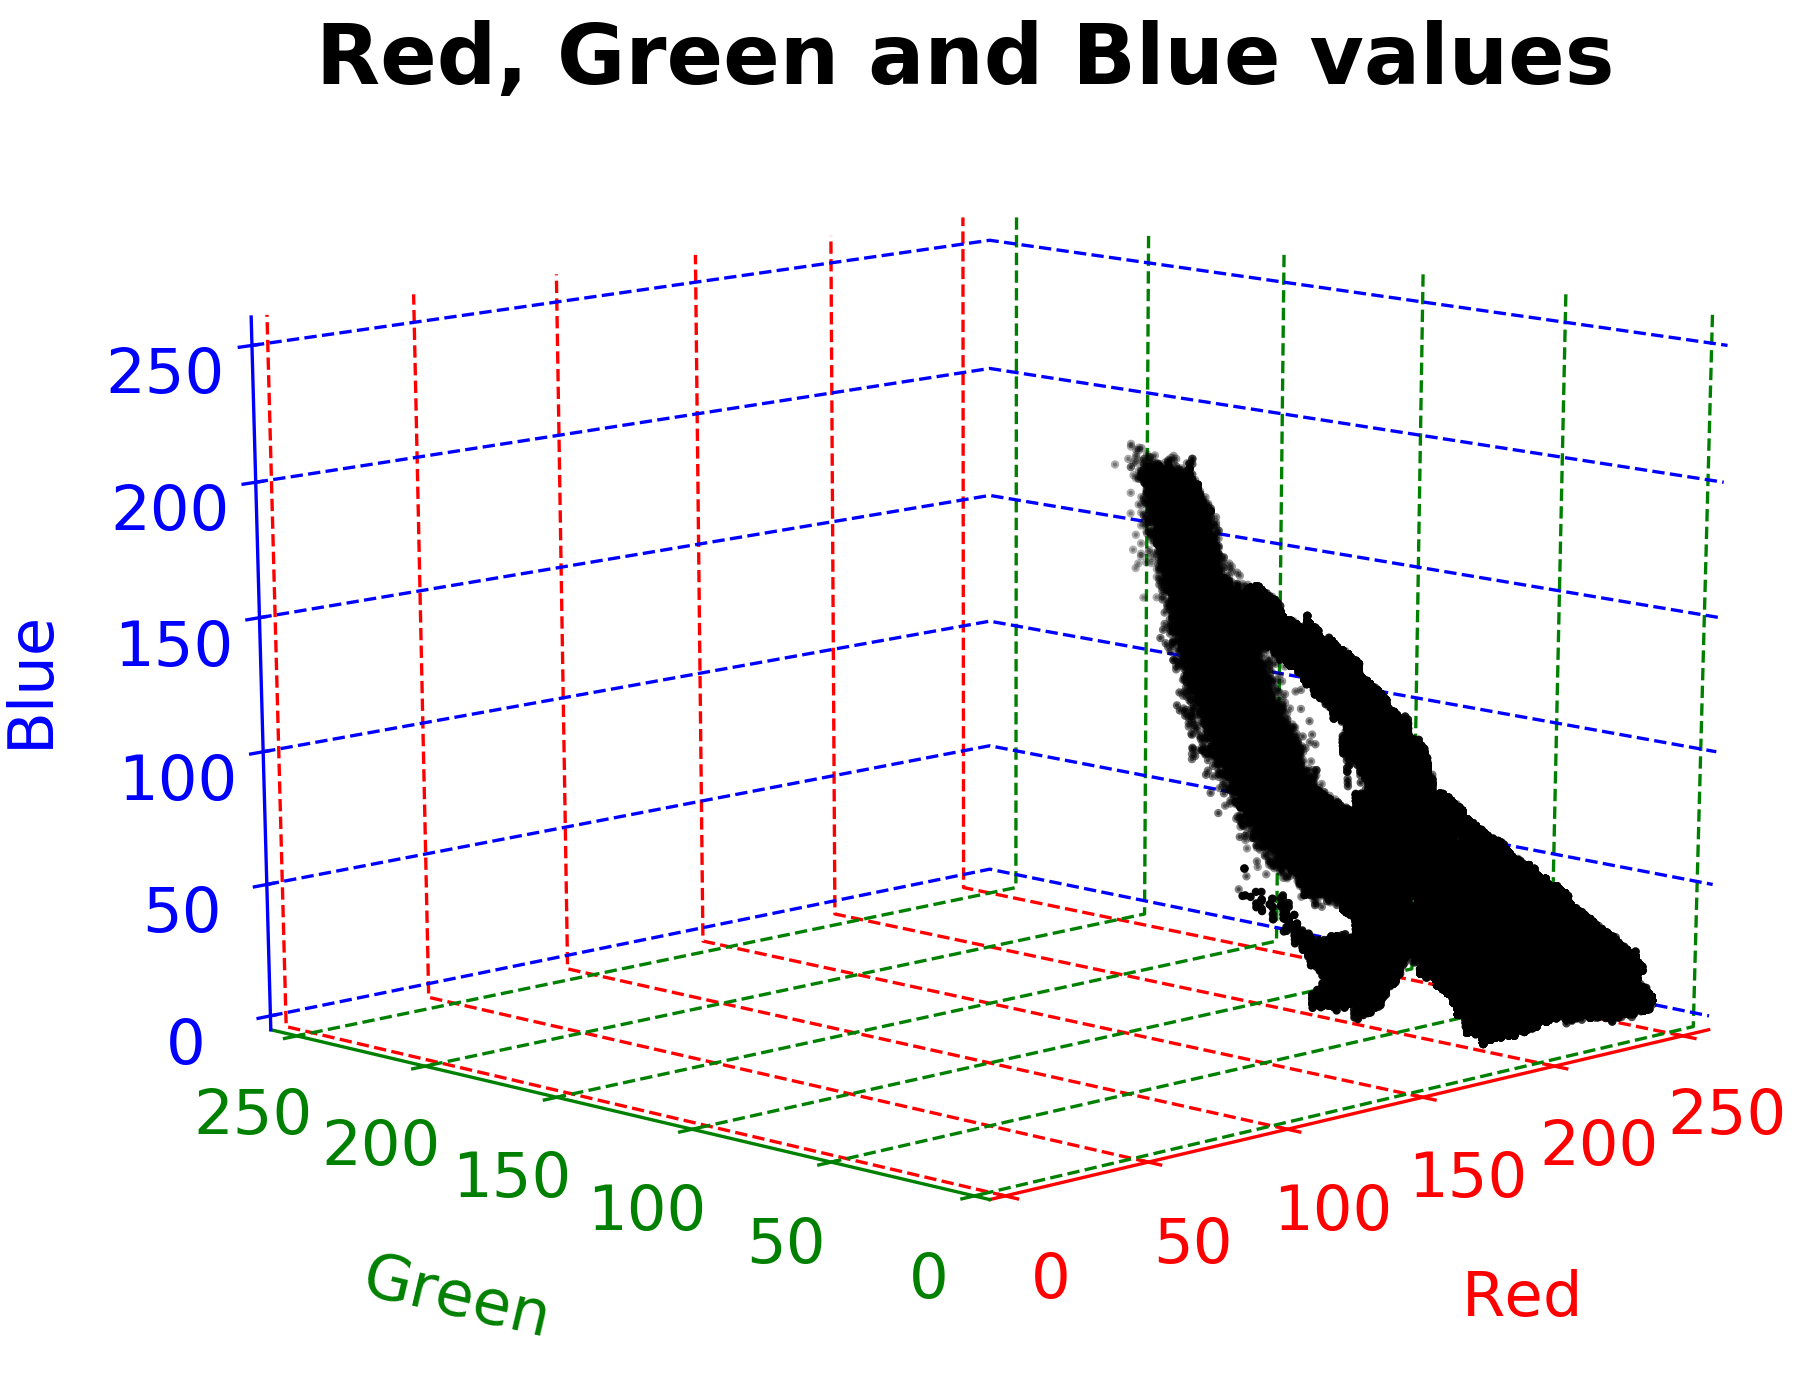
\includegraphics[width=0.9\textwidth]{img/rgbRed.png}
		\captionsetup{width=0.9\textwidth}
		\captionof{figure}{RGB plot voor de kleur rood.}
		\label{rgbRedPlot}
	\end{minipage}%
	\begin{minipage}{0.5\textwidth}
		\centering
		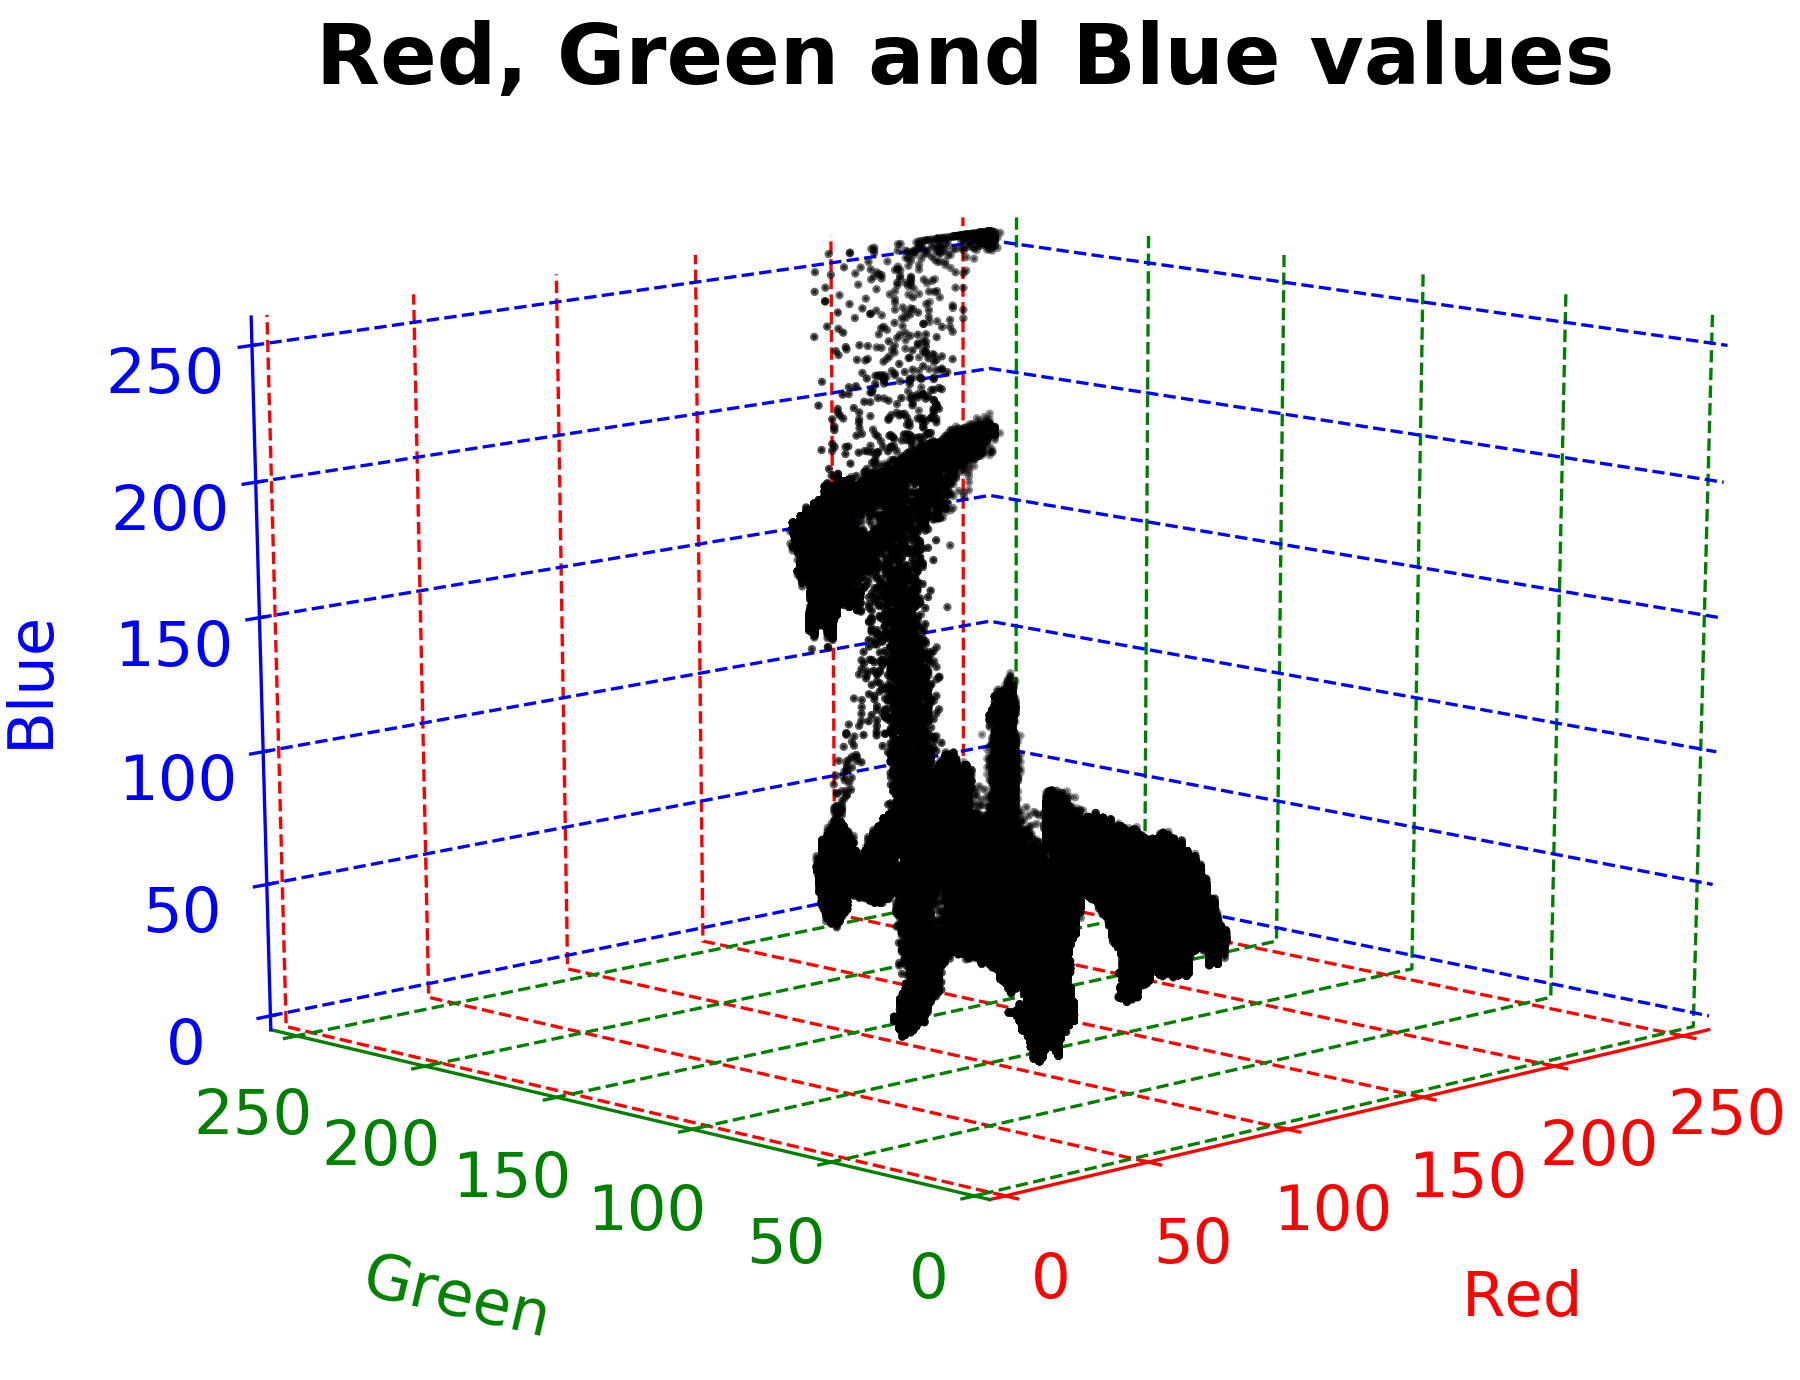
\includegraphics[width=0.9\textwidth]{img/rgbYellow.png}
		\captionsetup{width=0.9\textwidth}
		\captionof{figure}{RGB plot voor de kleur geel.}
		\label{rgbYellowPlot}
	\end{minipage}
\end{figure}

\vspace{1mm}

\begin{figure}[h!]
	\centering
	\begin{minipage}{0.5\textwidth}
		\centering
		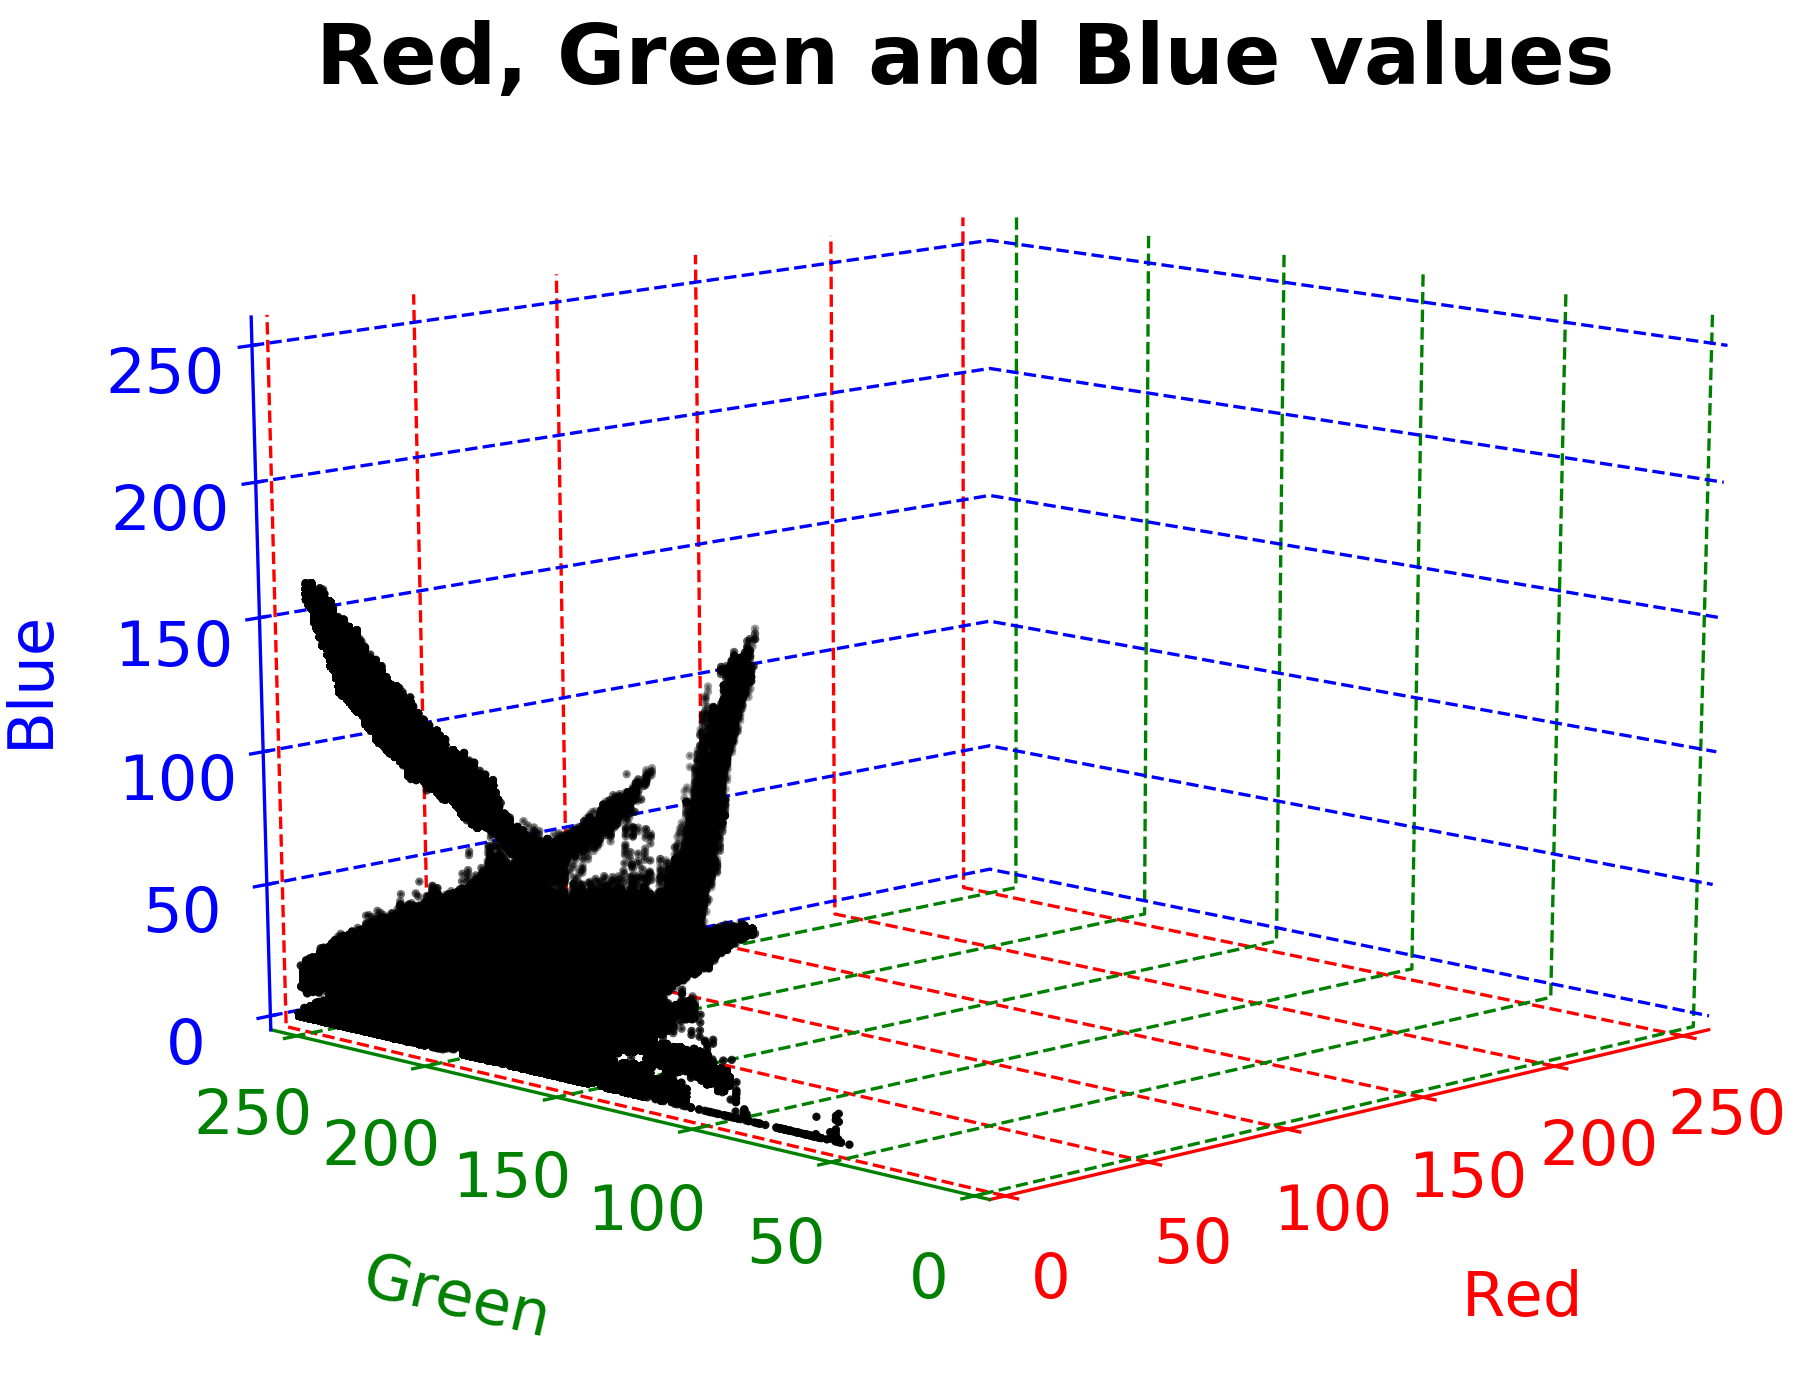
\includegraphics[width=0.9\textwidth]{img/rgbGreen.png}
		\captionsetup{width=0.9\textwidth}
		\captionof{figure}{RGB plot voor de kleur groen.}
		\label{rgbGreenPlot}
	\end{minipage}%
	\begin{minipage}{0.5\textwidth}
		\centering
		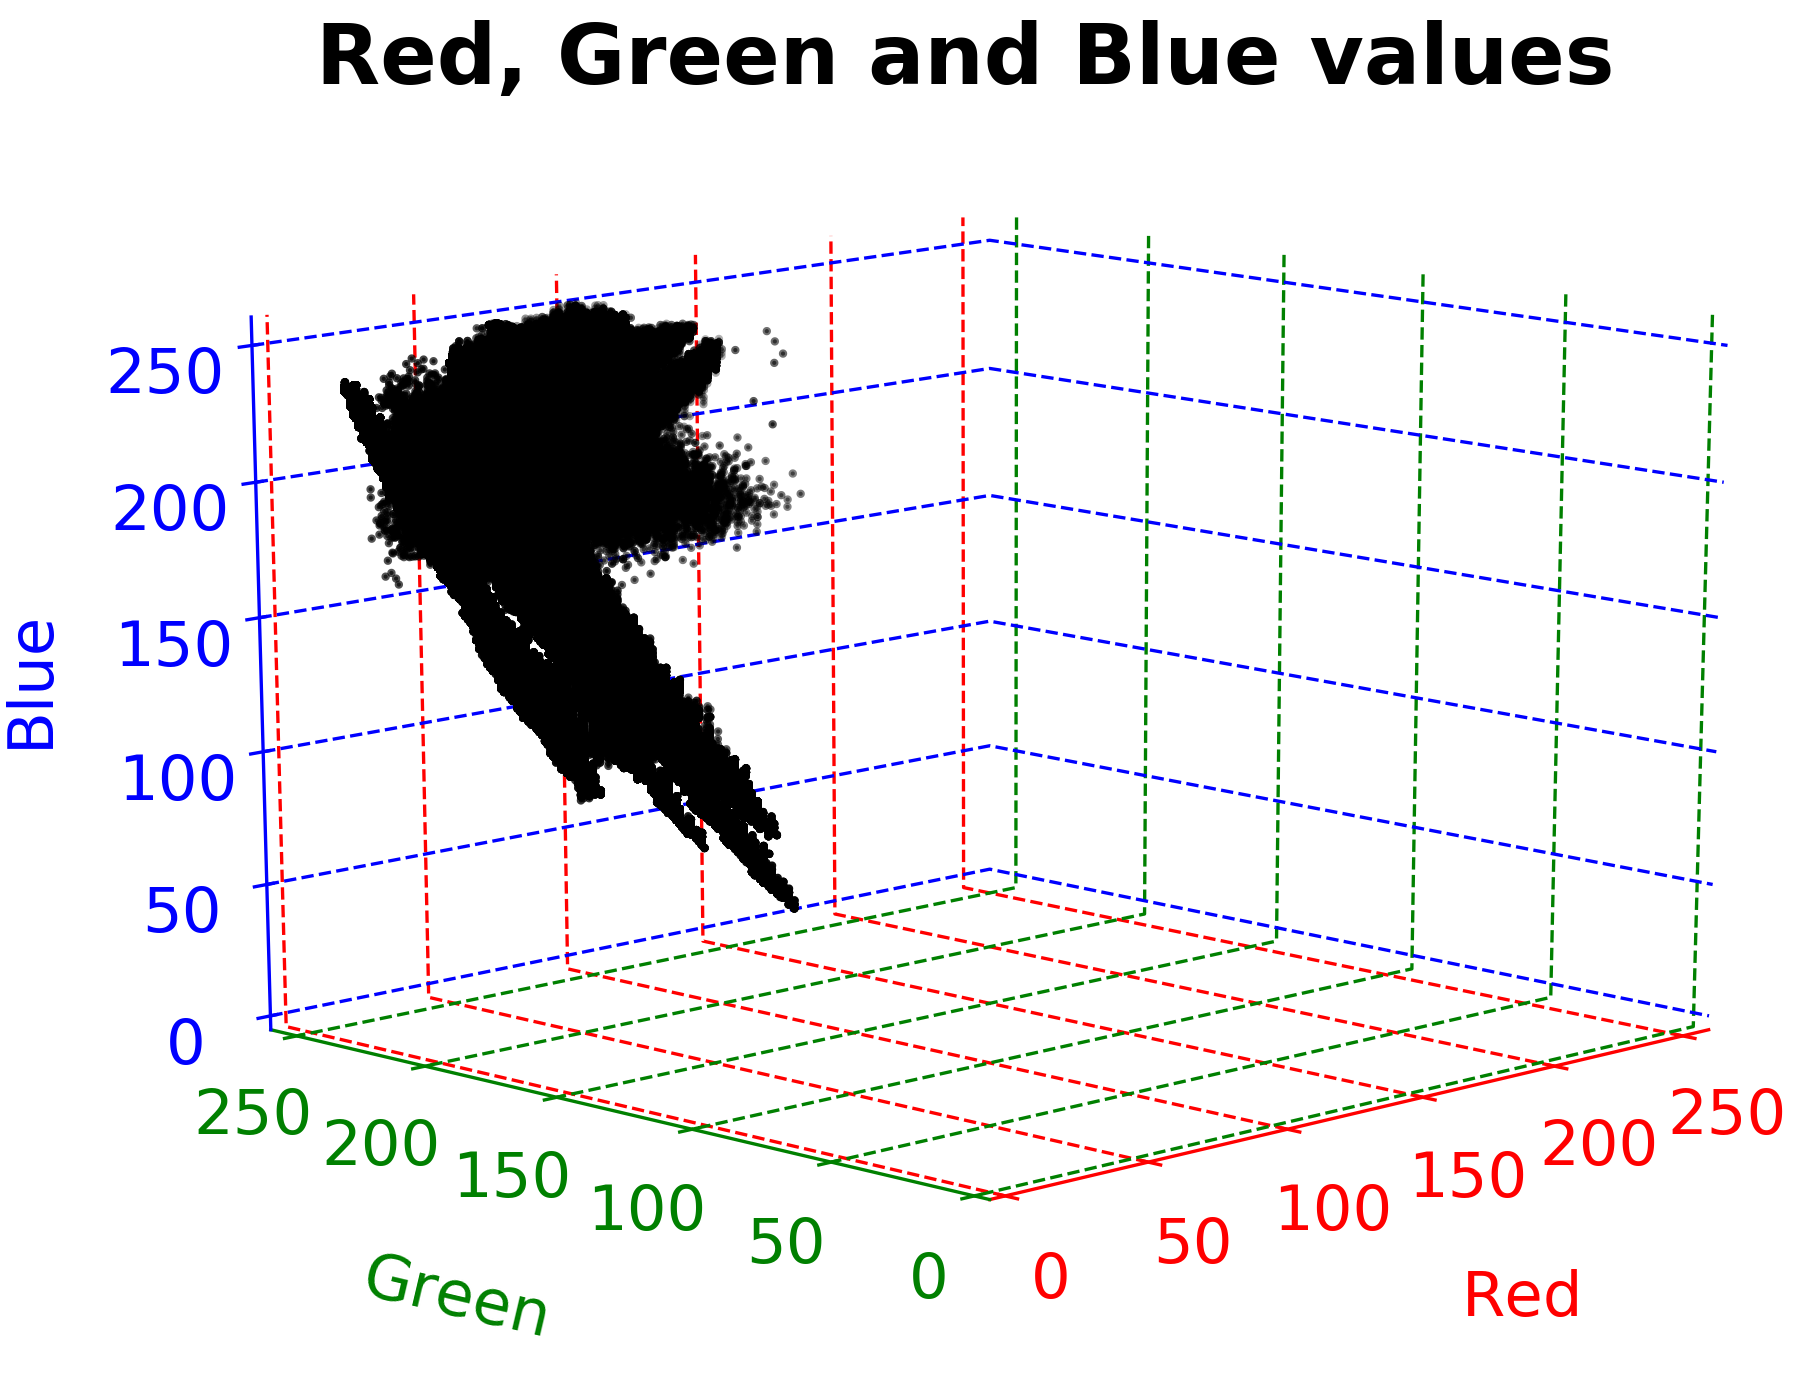
\includegraphics[width=0.9\textwidth]{img/rgbBlueGreen.png}
		\captionsetup{width=0.9\textwidth}
		\captionof{figure}{RGB plot voor de kleur cyaan.}
		\label{rgbBlueGreenPlot}
	\end{minipage}
\end{figure}

\vspace{1mm}

\begin{figure}[h!]
	\centering
	\begin{minipage}{0.5\textwidth}
		\centering
		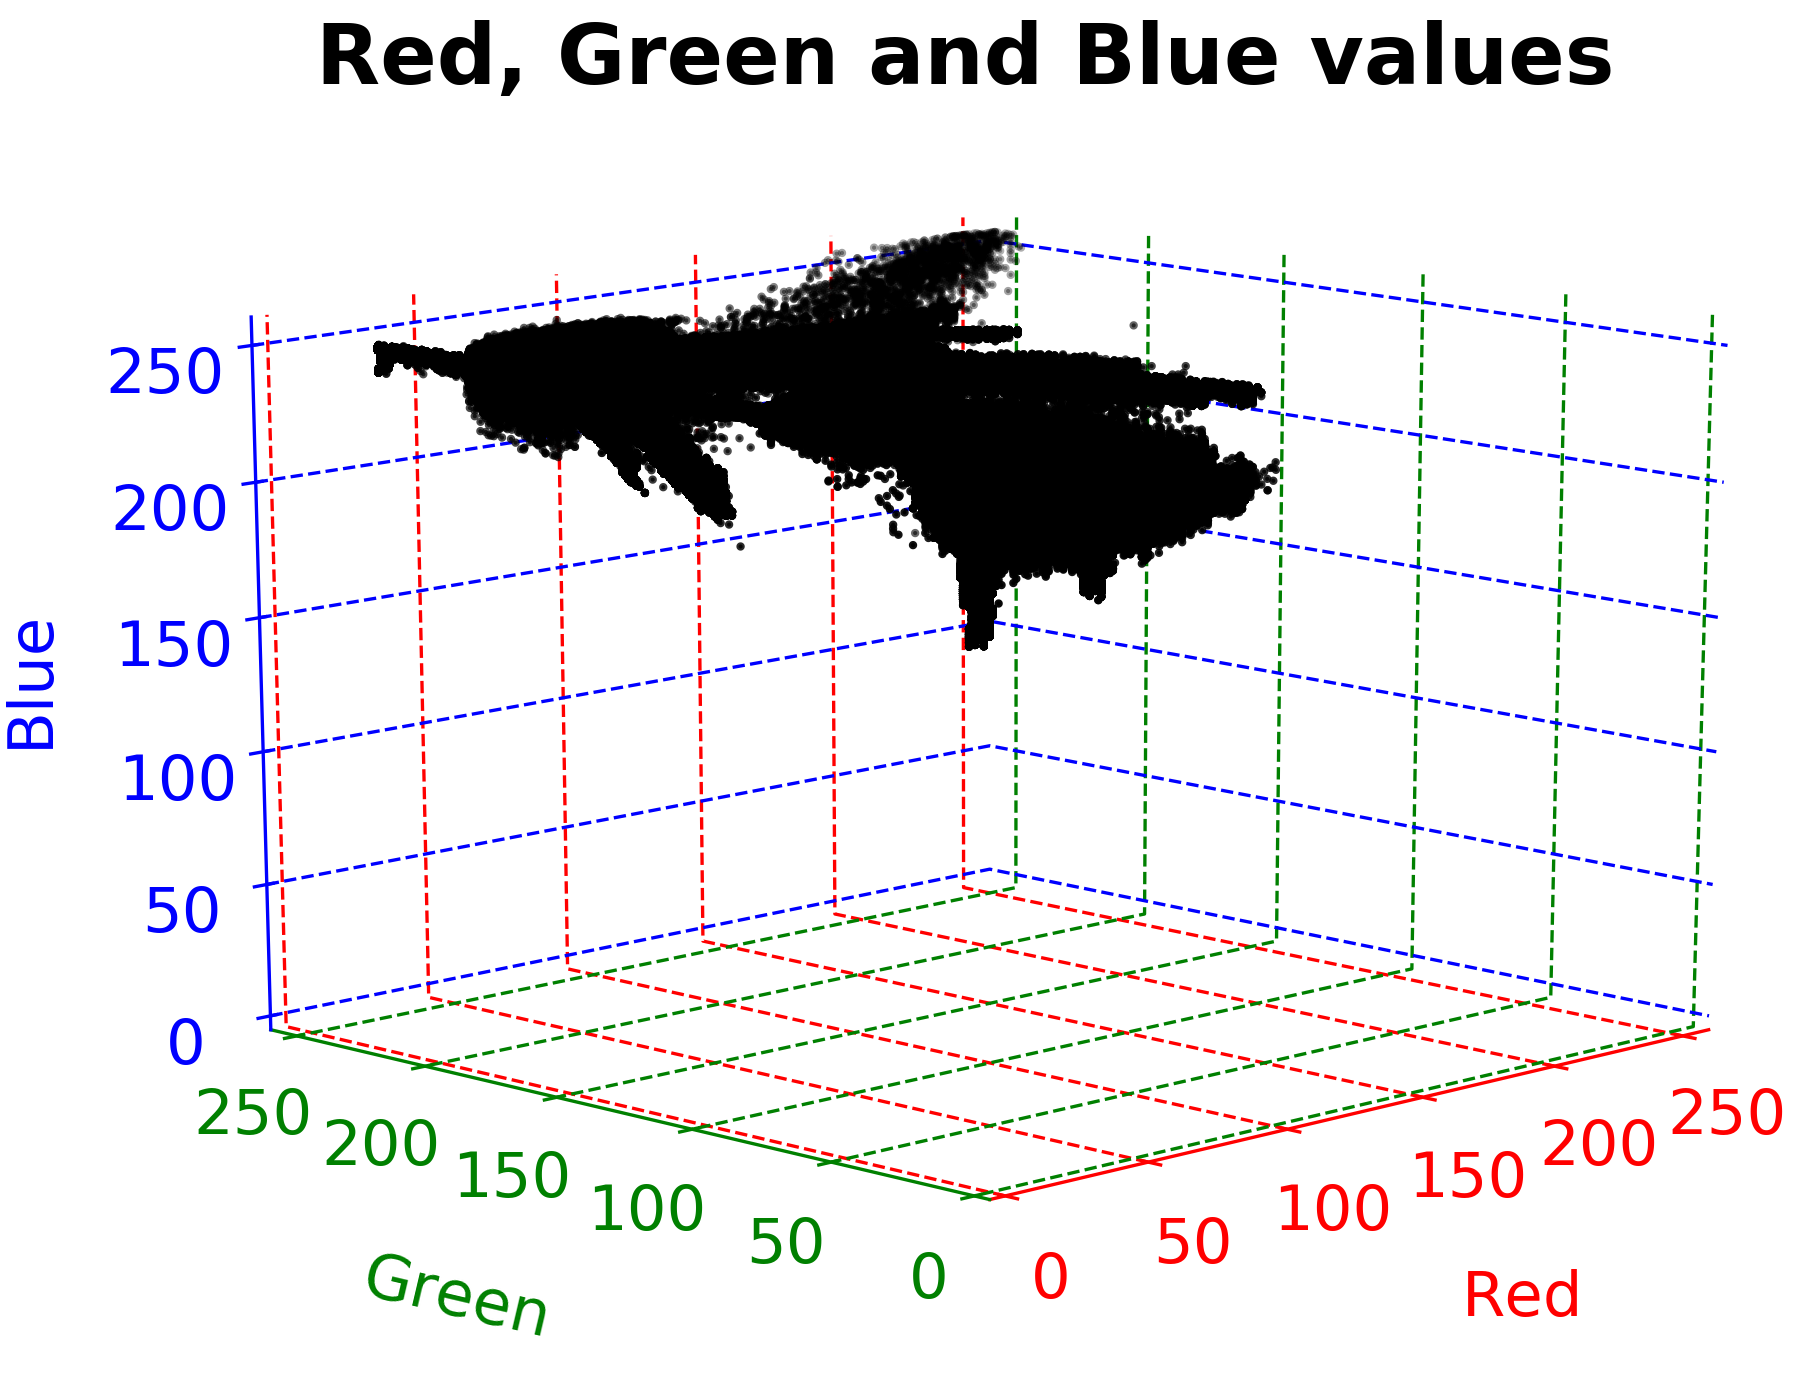
\includegraphics[width=0.9\textwidth]{img/rgbBlue.png}
		\captionsetup{width=0.9\textwidth}
		\captionof{figure}{RGB plot voor de kleur blauw.}
		\label{rgbBluePlot}
	\end{minipage}%	
	\begin{minipage}{0.5\textwidth}
		\centering
		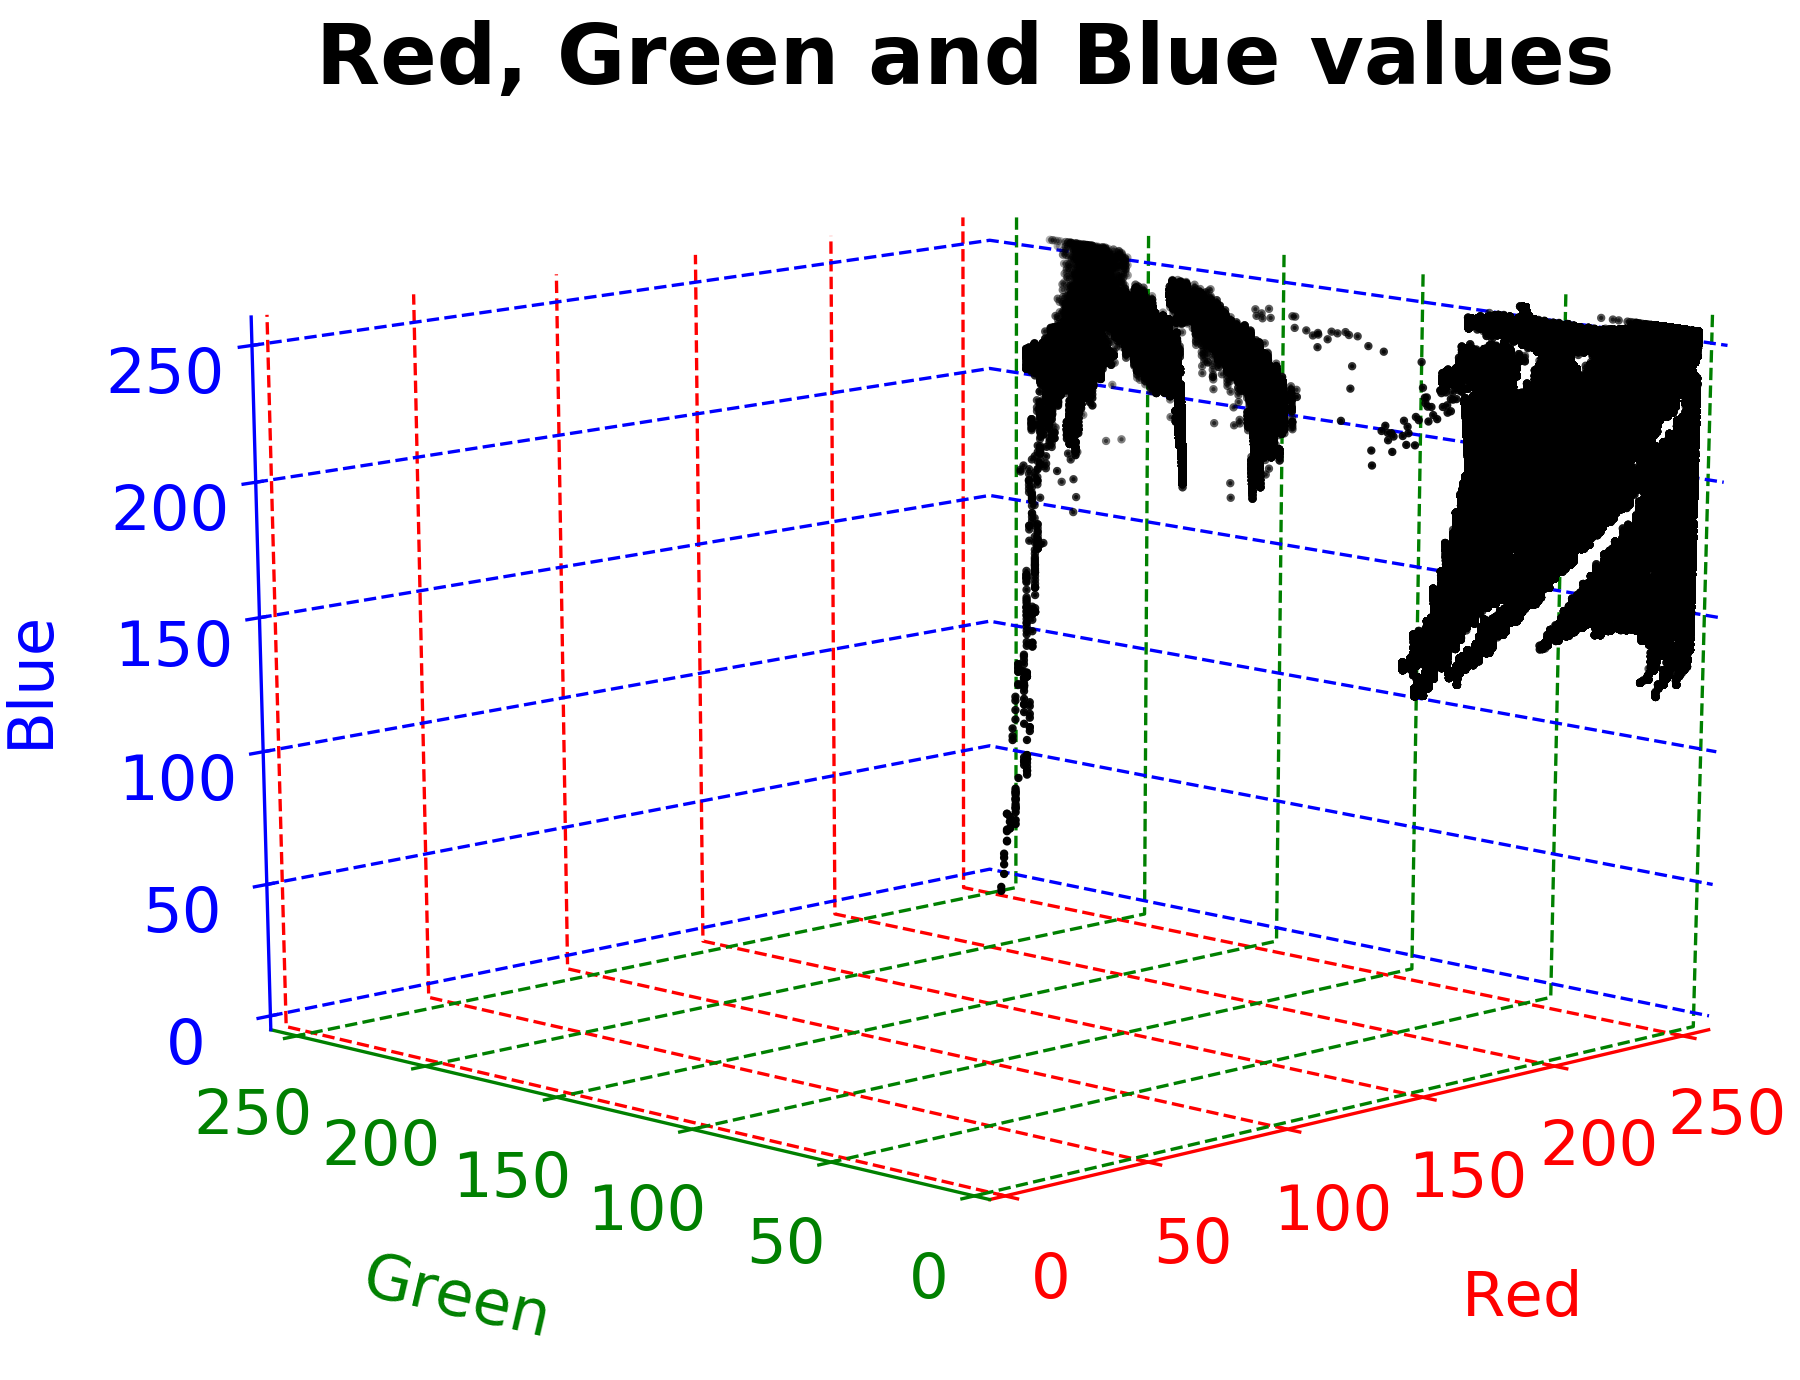
\includegraphics[width=0.9\textwidth]{img/rgbPink.png}
		\captionsetup{width=0.9\textwidth}
		\captionof{figure}{RGB plot voor de kleur magenta.}
		\label{rgbPinkPlot}
	\end{minipage}
\end{figure}

\subsection{Histogrammen}

\begin{figure}[h!]
	\centering
	\begin{minipage}{0.5\textwidth}
		\centering
		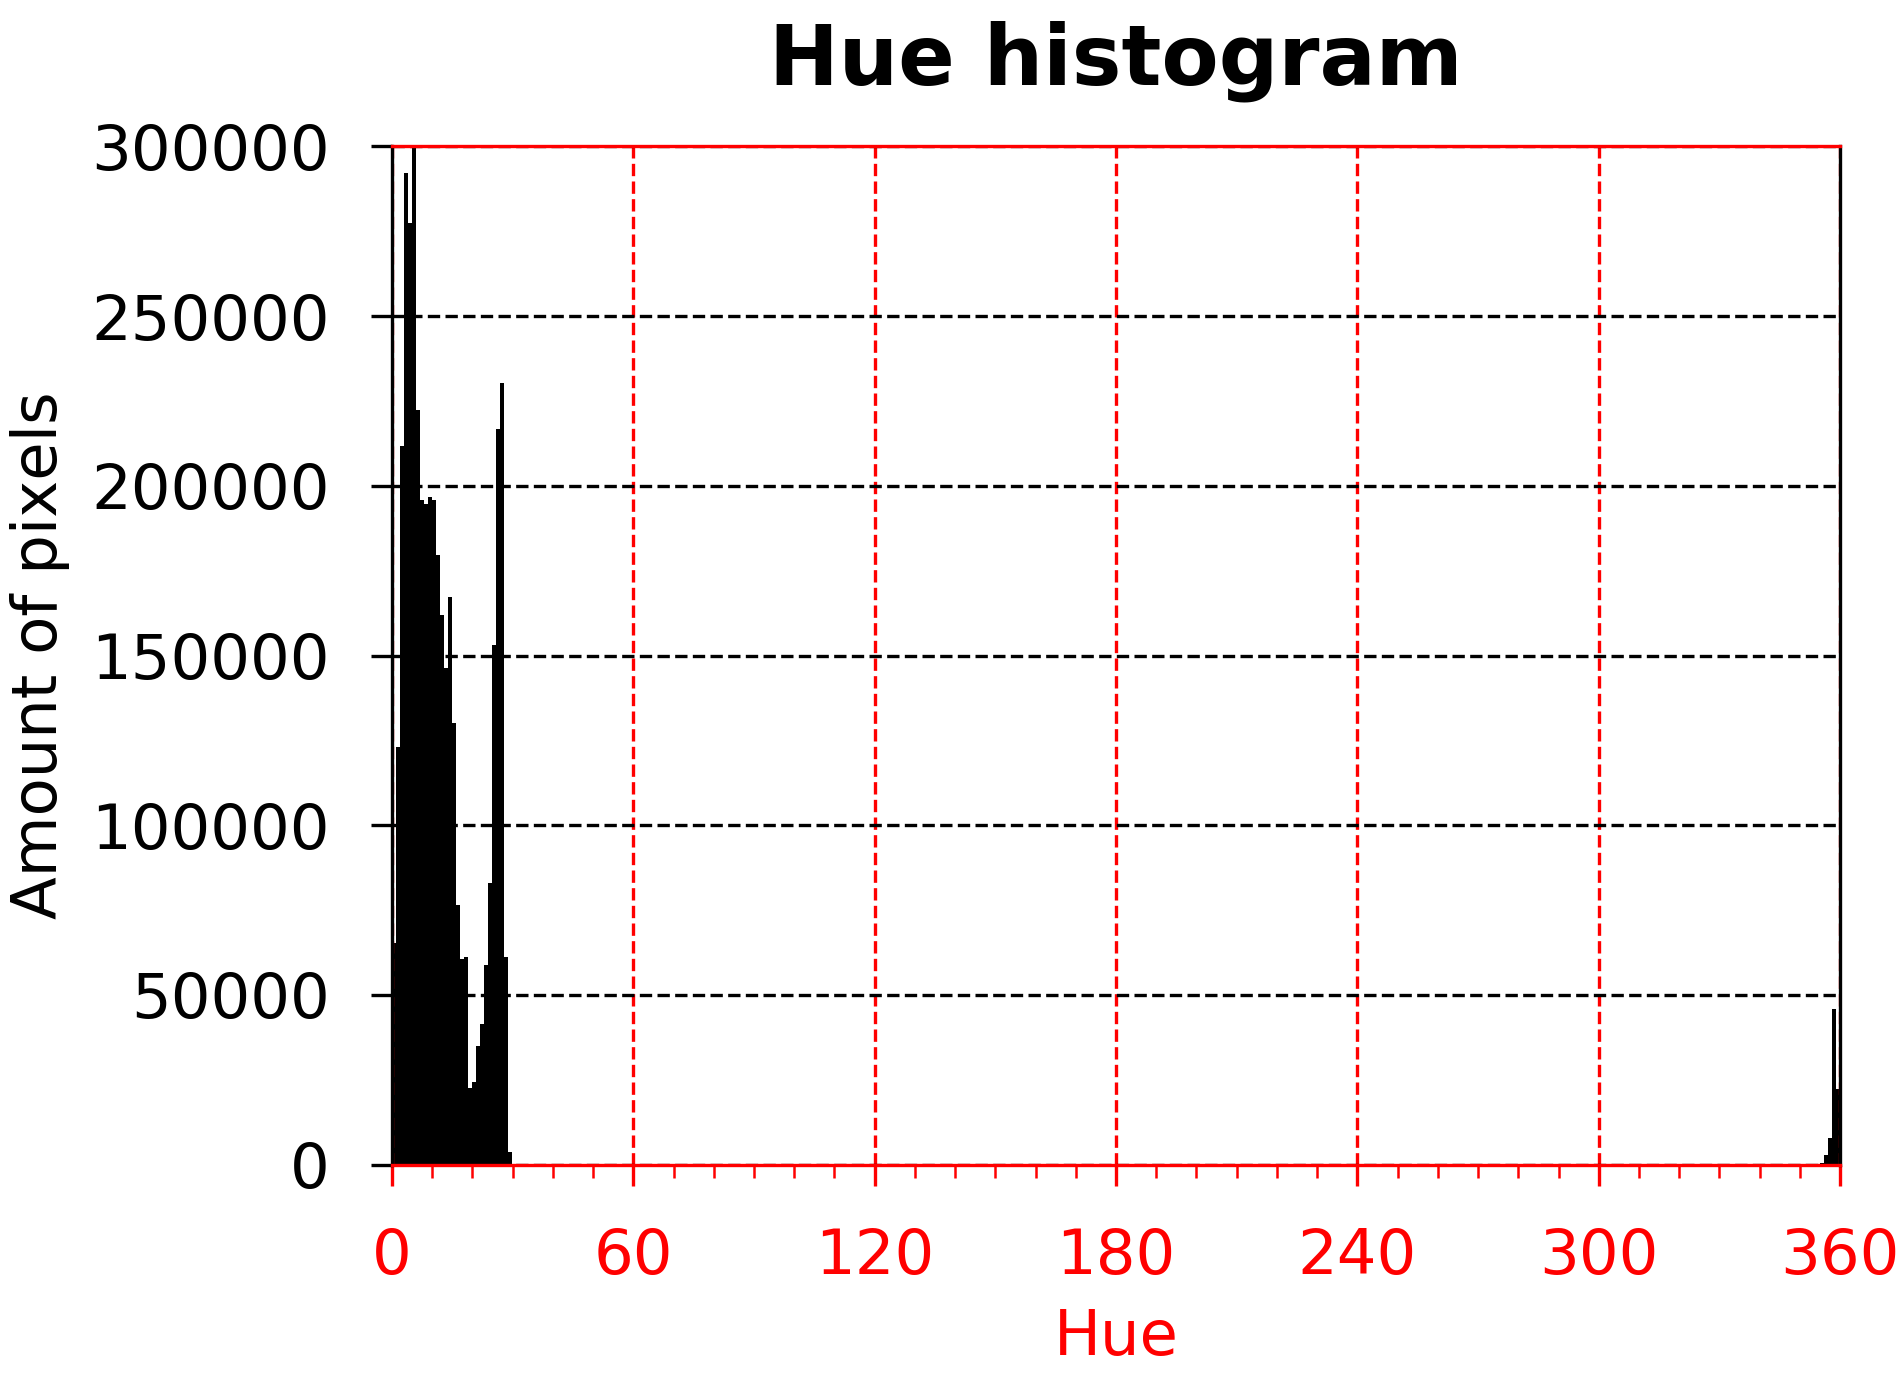
\includegraphics[width=0.9\textwidth]{img/hueHistRed.png}
		\captionsetup{width=0.9\textwidth}
		\captionof{figure}{Histogram van de tint in functie van het aantal waargenomen pixels voor de kleur rood.}
		\label{histRed}
	\end{minipage}%
	\begin{minipage}{0.5\textwidth}
		\centering
		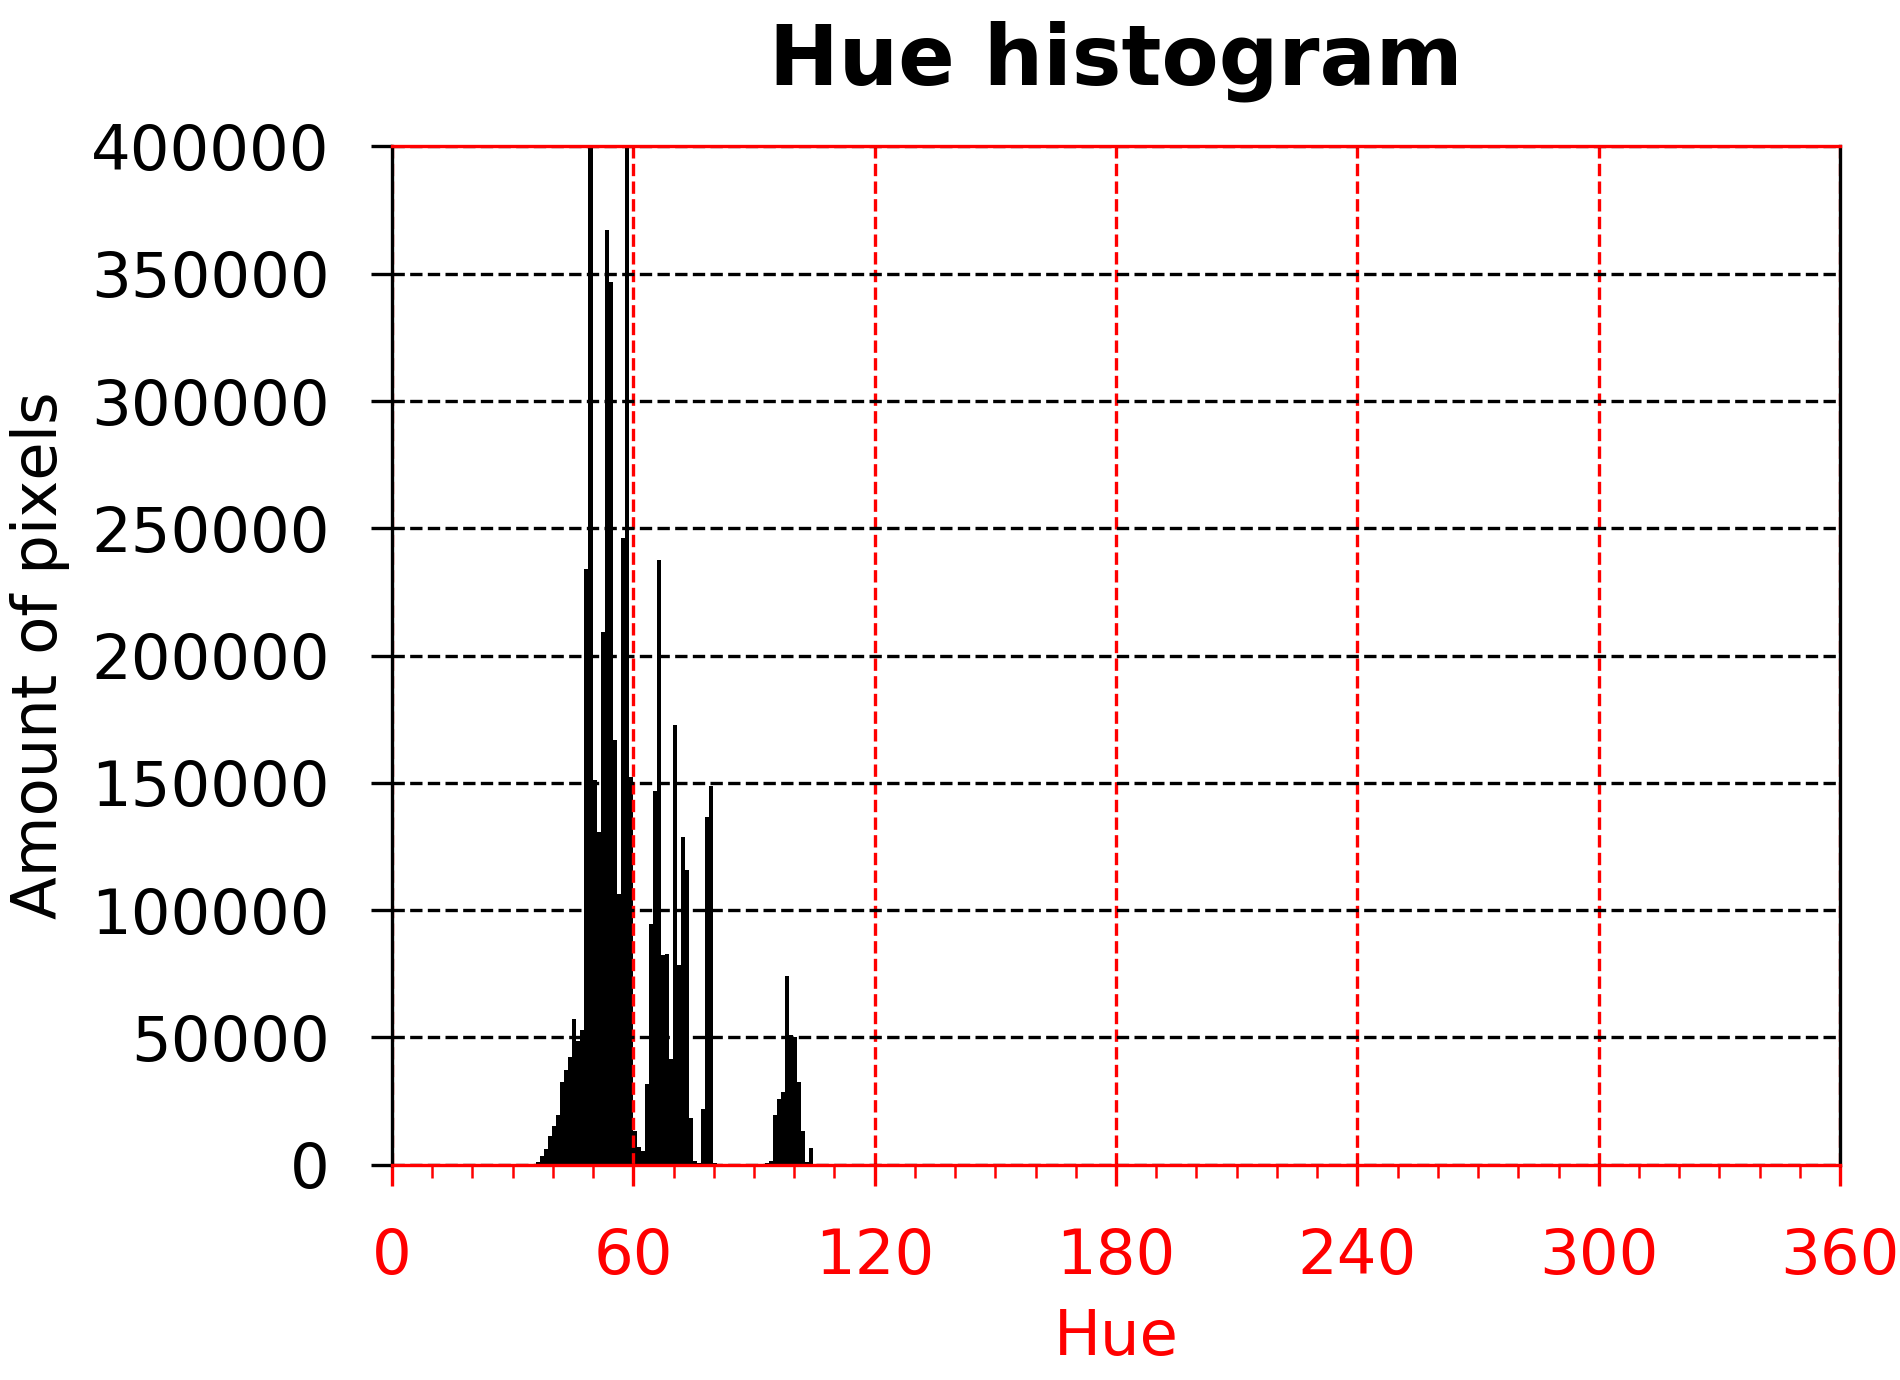
\includegraphics[width=0.9\textwidth]{img/hueHistYellow.png}
		\captionsetup{width=0.9\textwidth}
		\captionof{figure}{Histogram van de tint in functie van het aantal waargenomen pixels voor de kleur geel.}
	\label{histYellow}
	\end{minipage}
\end{figure}

\vspace{1mm}

\begin{figure}[h!]
	\centering
	\begin{minipage}{0.5\textwidth}
		\centering
		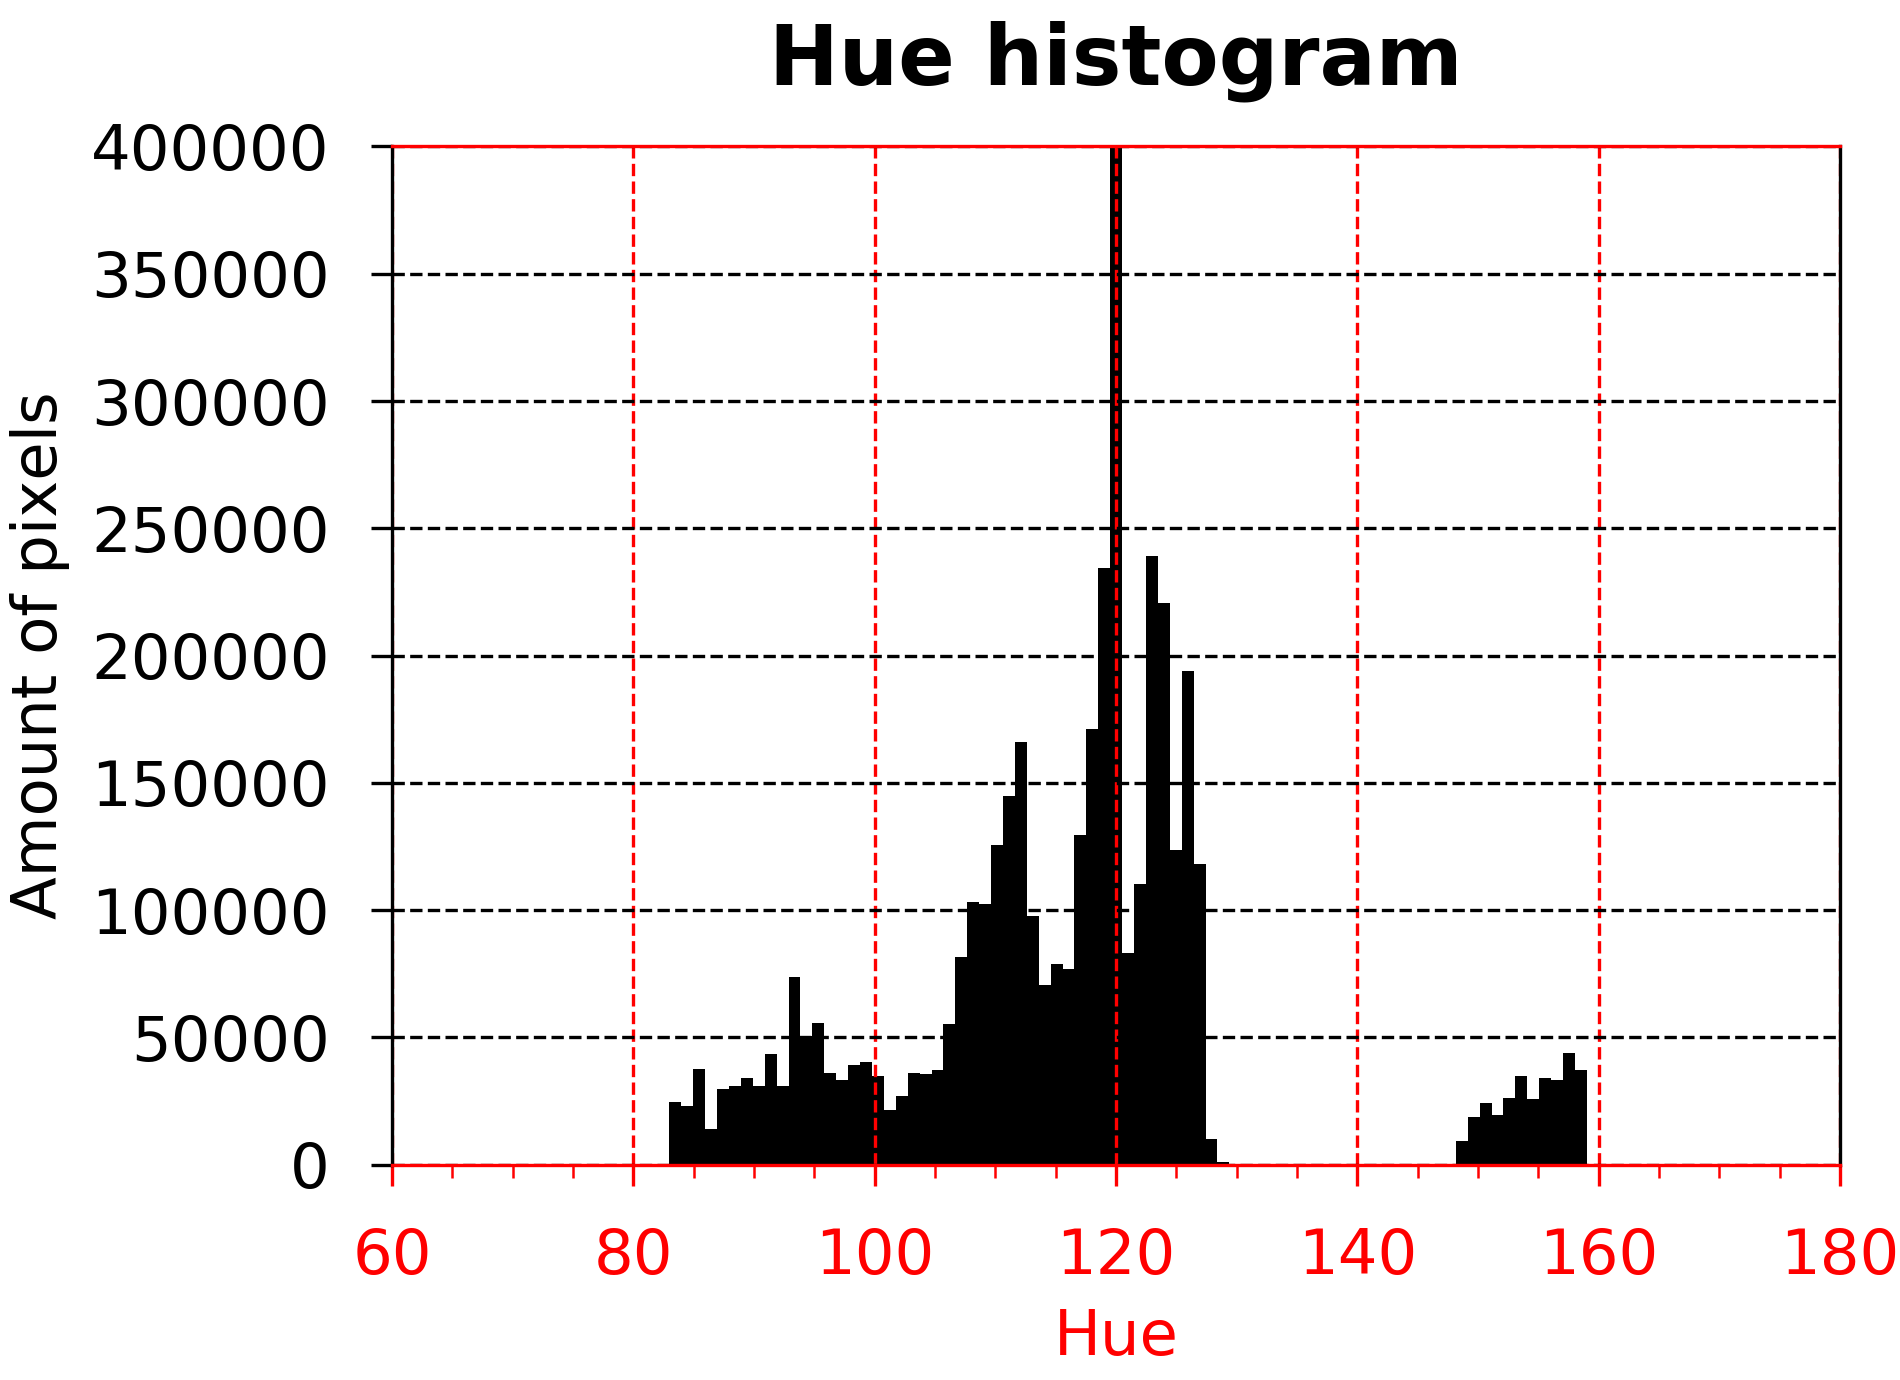
\includegraphics[width=0.9\textwidth]{img/hueHistGreen.png}
		\captionsetup{width=0.9\textwidth}
		\captionof{figure}{Histogram van de tint in functie van het aantal waargenomen pixels voor de kleur groen.}
		\label{histGreen}
	\end{minipage}%
	\begin{minipage}{0.5\textwidth}
		\centering
		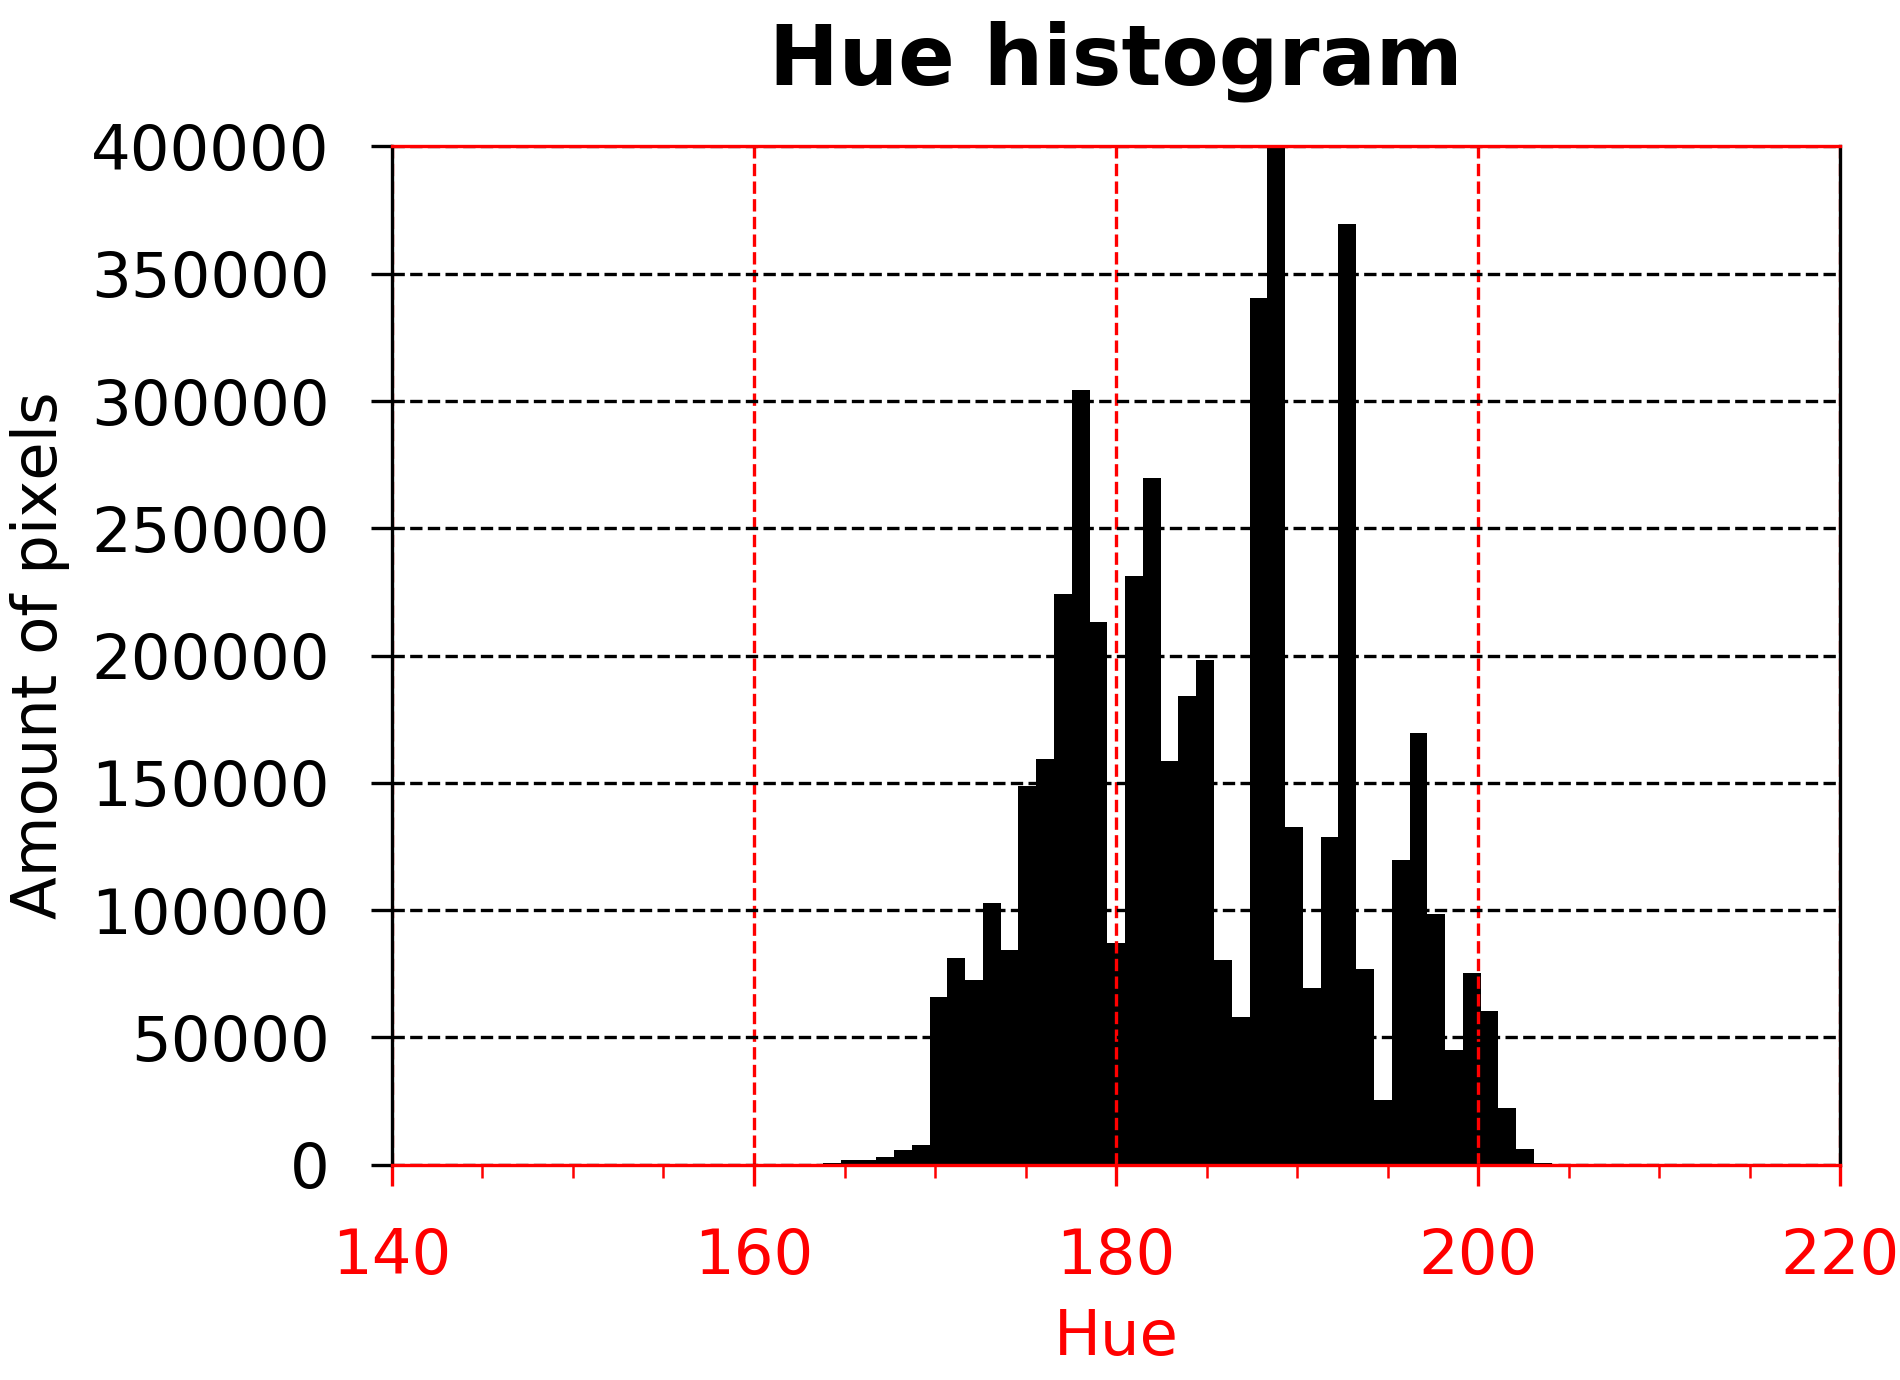
\includegraphics[width=0.9\textwidth]{img/hueHistBlueGreen.png}
		\captionsetup{width=0.9\textwidth}
		\captionof{figure}{Histogram van de tint in functie van het aantal waargenomen pixels voor de kleur cyaan.}
	\label{histBluegreen}
	\end{minipage}
\end{figure}

\vspace{1mm}

\begin{figure}[h!]
	\centering
	\begin{minipage}{0.5\textwidth}
		\centering
		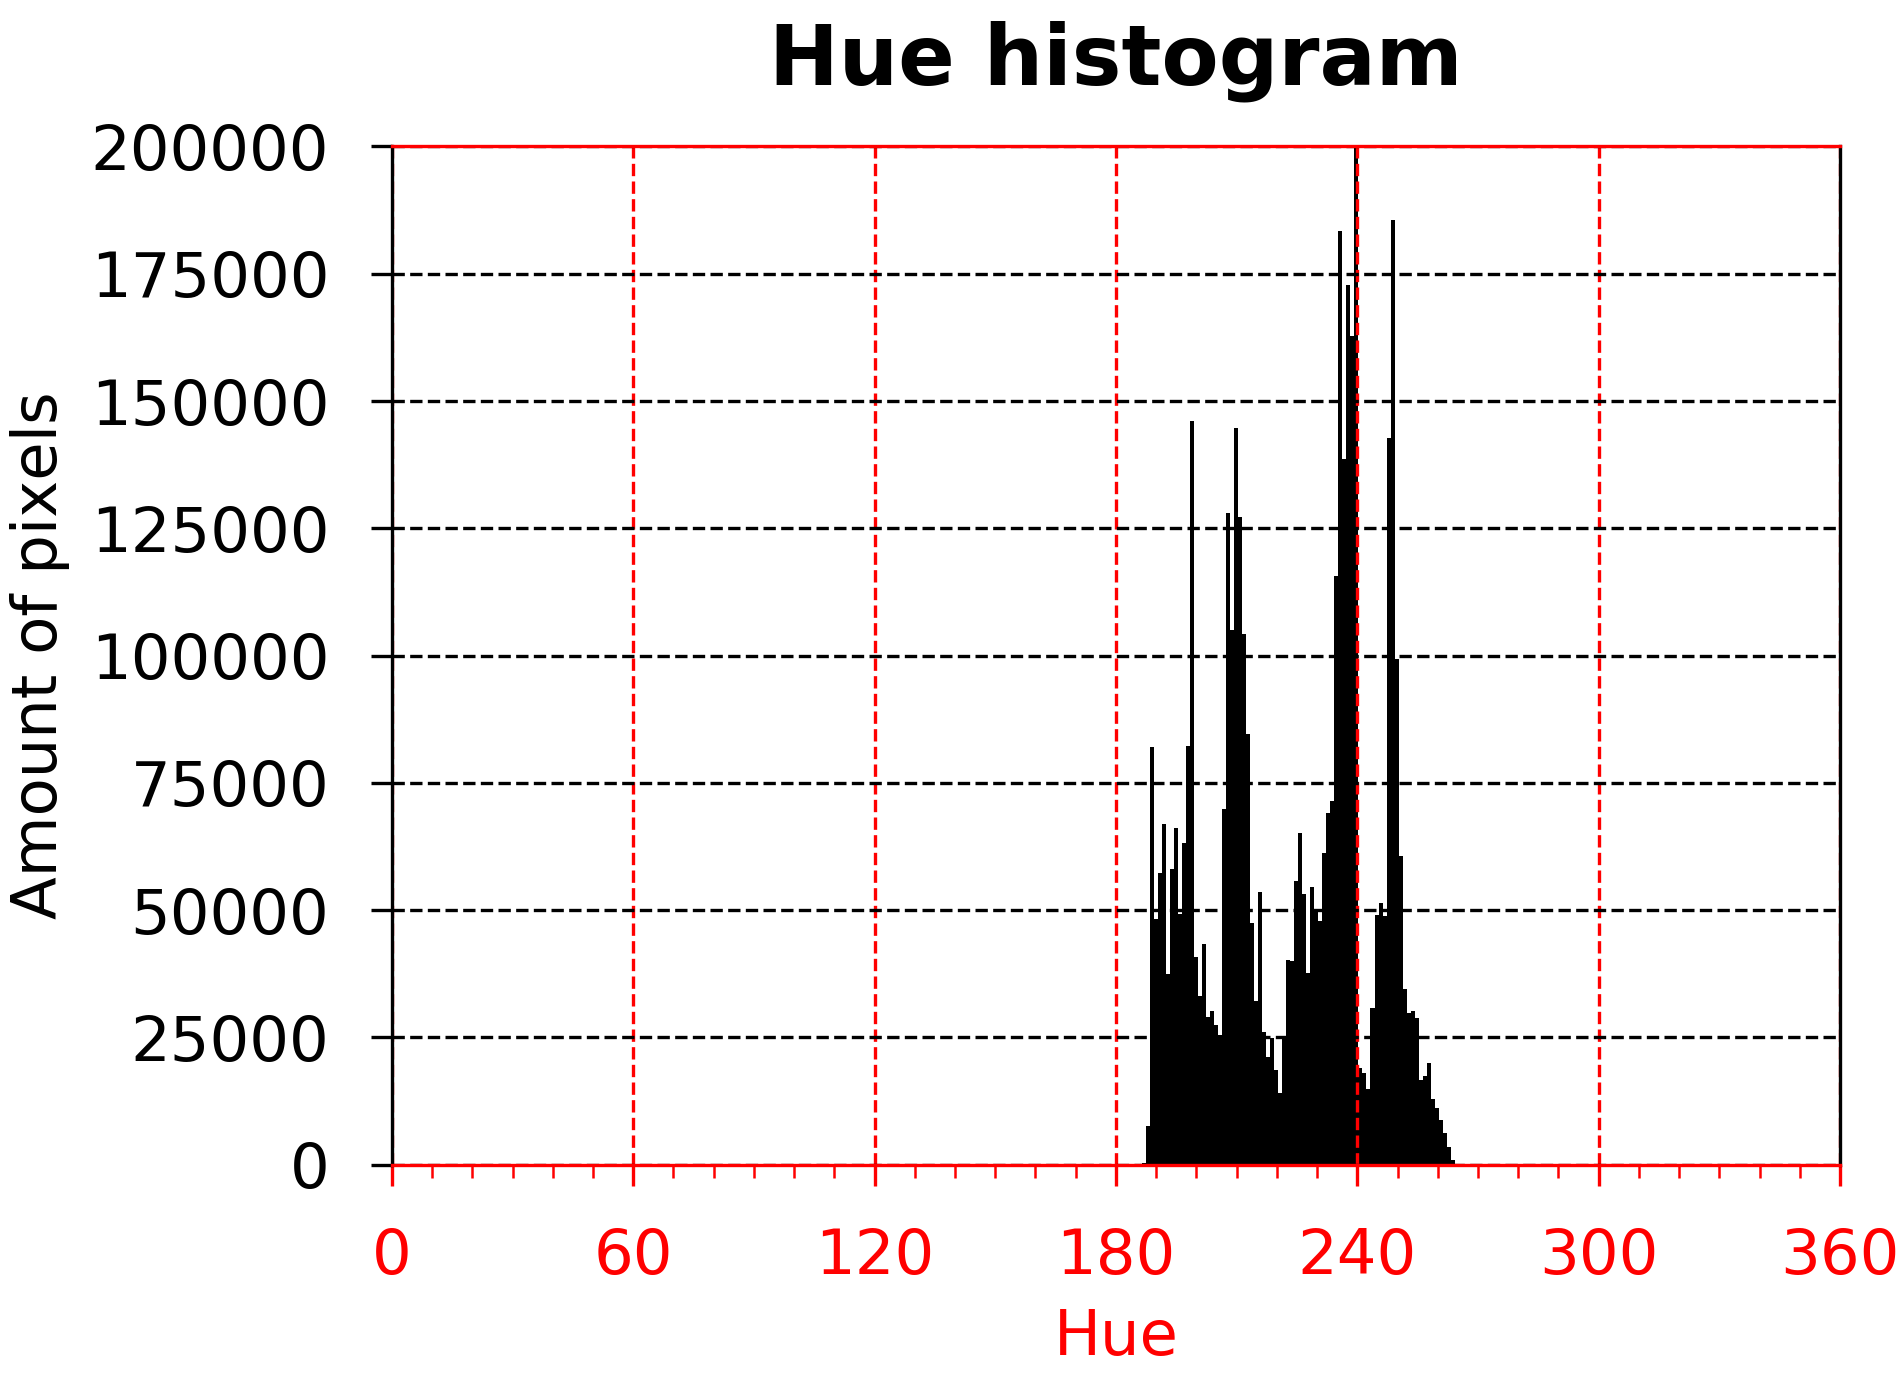
\includegraphics[width=0.9\textwidth]{img/hueHistBlue.png}
		\captionsetup{width=0.9\textwidth}
		\captionof{figure}{Histogram van de tint in functie van het aantal waargenomen pixels voor de kleur blauw.}
		\label{histBlue}
	\end{minipage}%
	\begin{minipage}{0.5\textwidth}
		\centering
		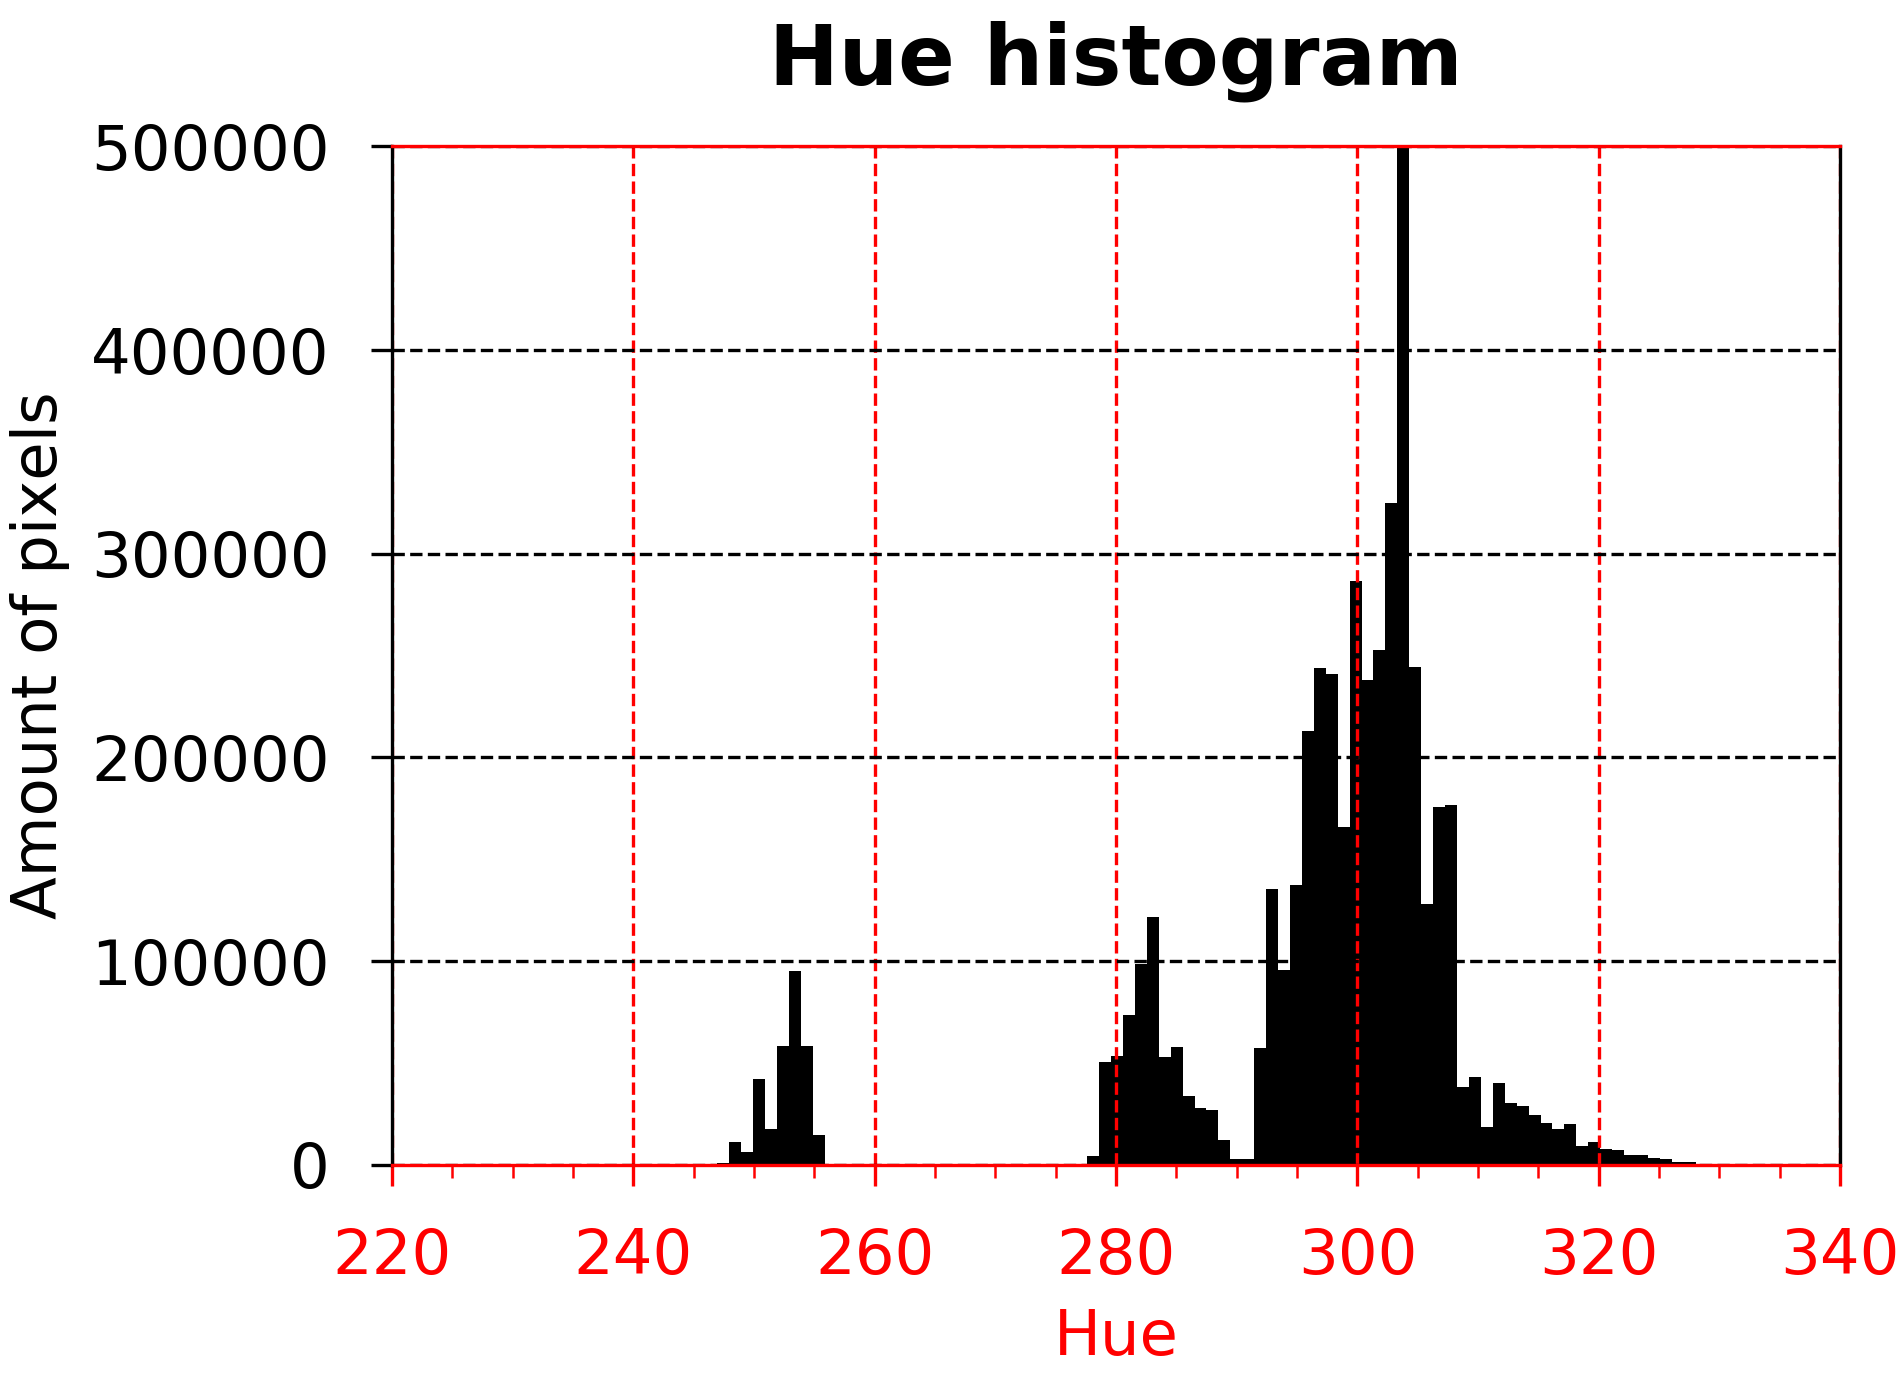
\includegraphics[width=0.9\textwidth]{img/hueHistPink.png}
		\captionsetup{width=0.9\textwidth}
		\captionof{figure}{Histogram van de tint in functie van het aantal waargenomen pixels voor de kleur magenta.}
	\label{histPink}
	\end{minipage}
\end{figure}

\subsection{HSL plots}

\subsubsection{3D}

\begin{figure}[h!]
	\centering
	\begin{minipage}{0.5\textwidth}
		\centering
		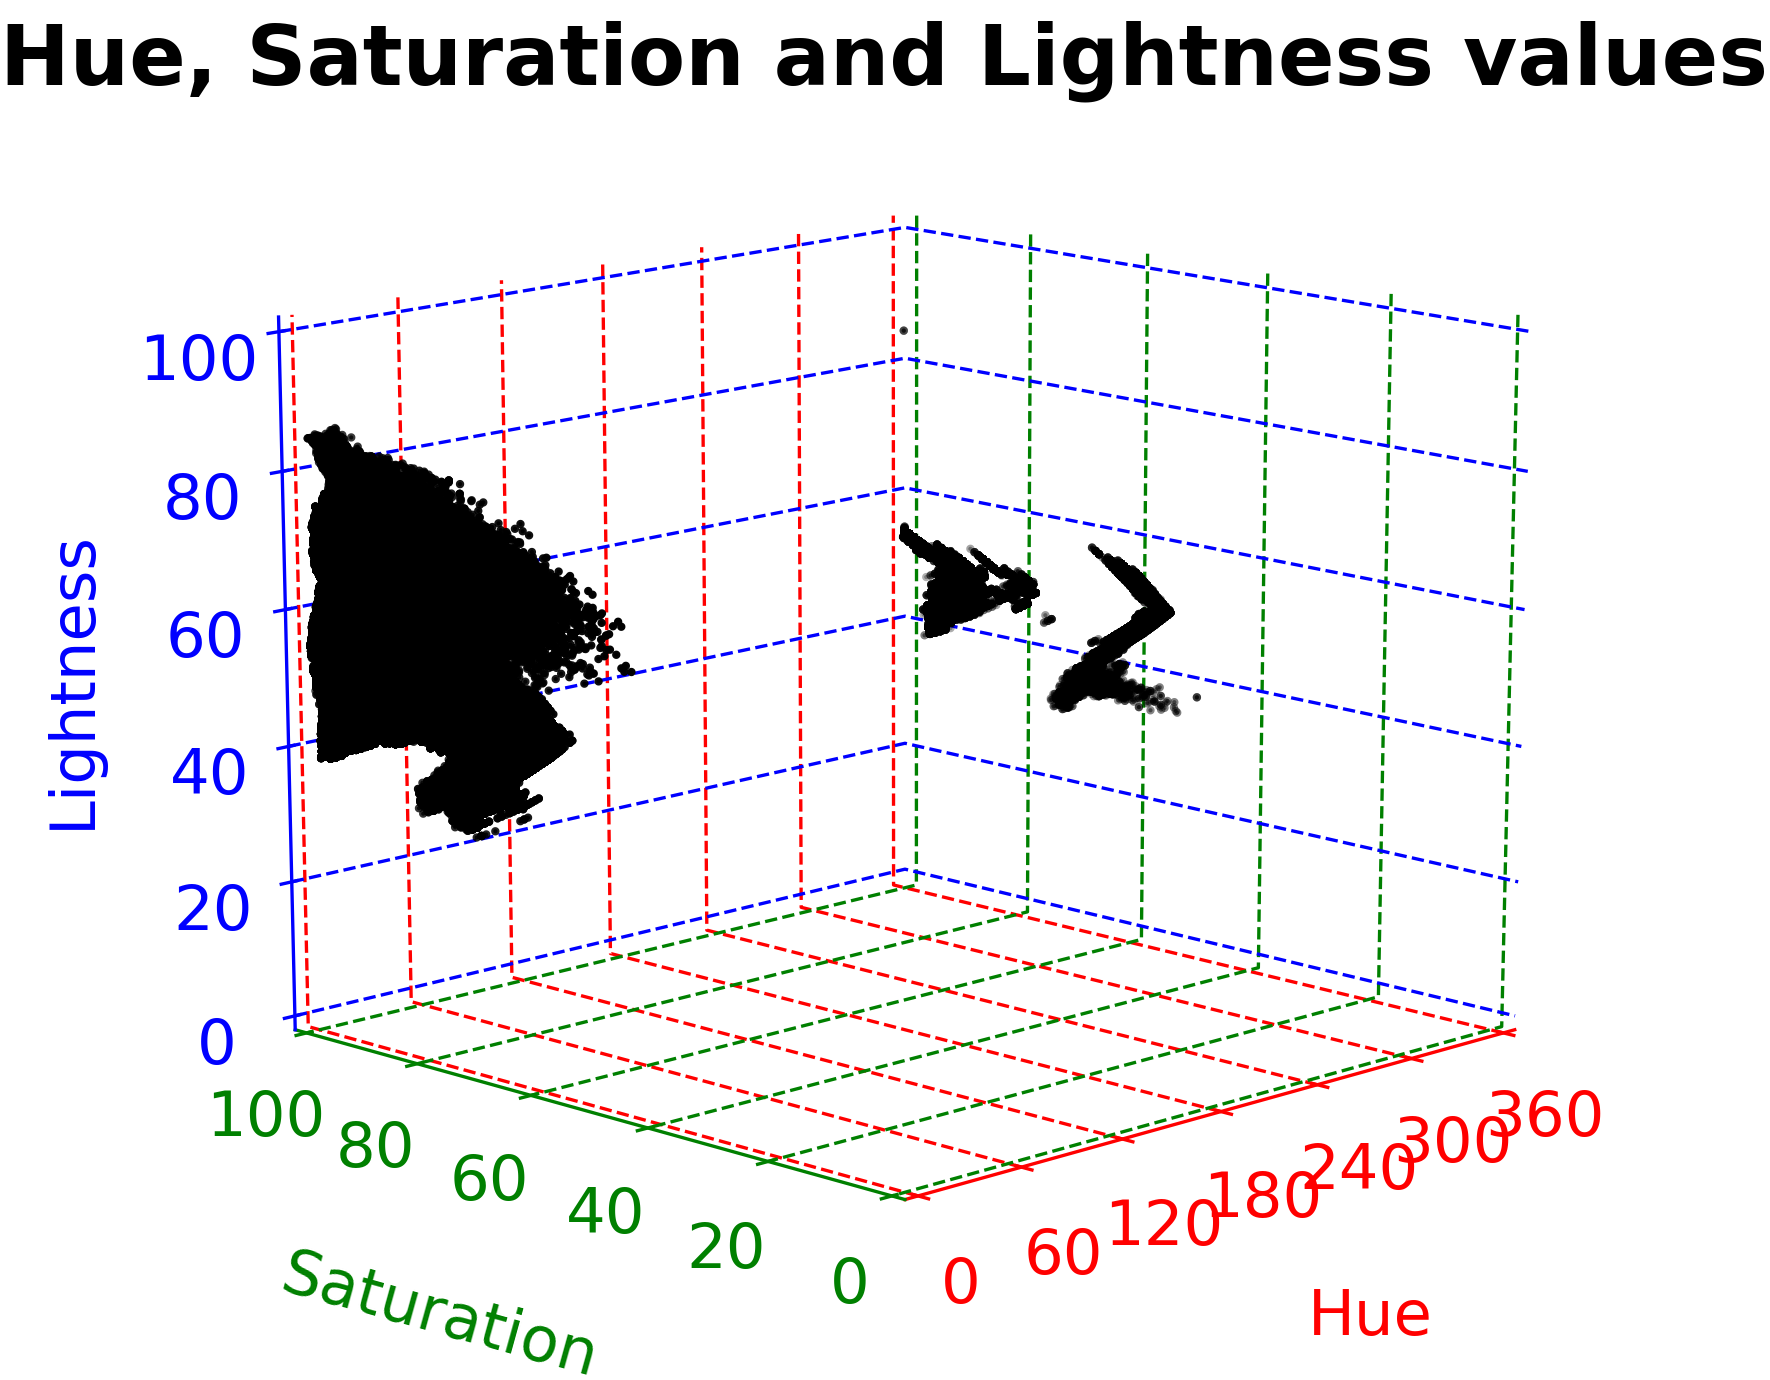
\includegraphics[width=0.9\textwidth]{img/hsl3DRed.png}
		\captionsetup{width=0.9\textwidth}
		\captionof{figure}{HSL plot voor de kleur rood.}
		\label{hsl3DRedPlot}
	\end{minipage}%
	\begin{minipage}{0.5\textwidth}
		\centering
		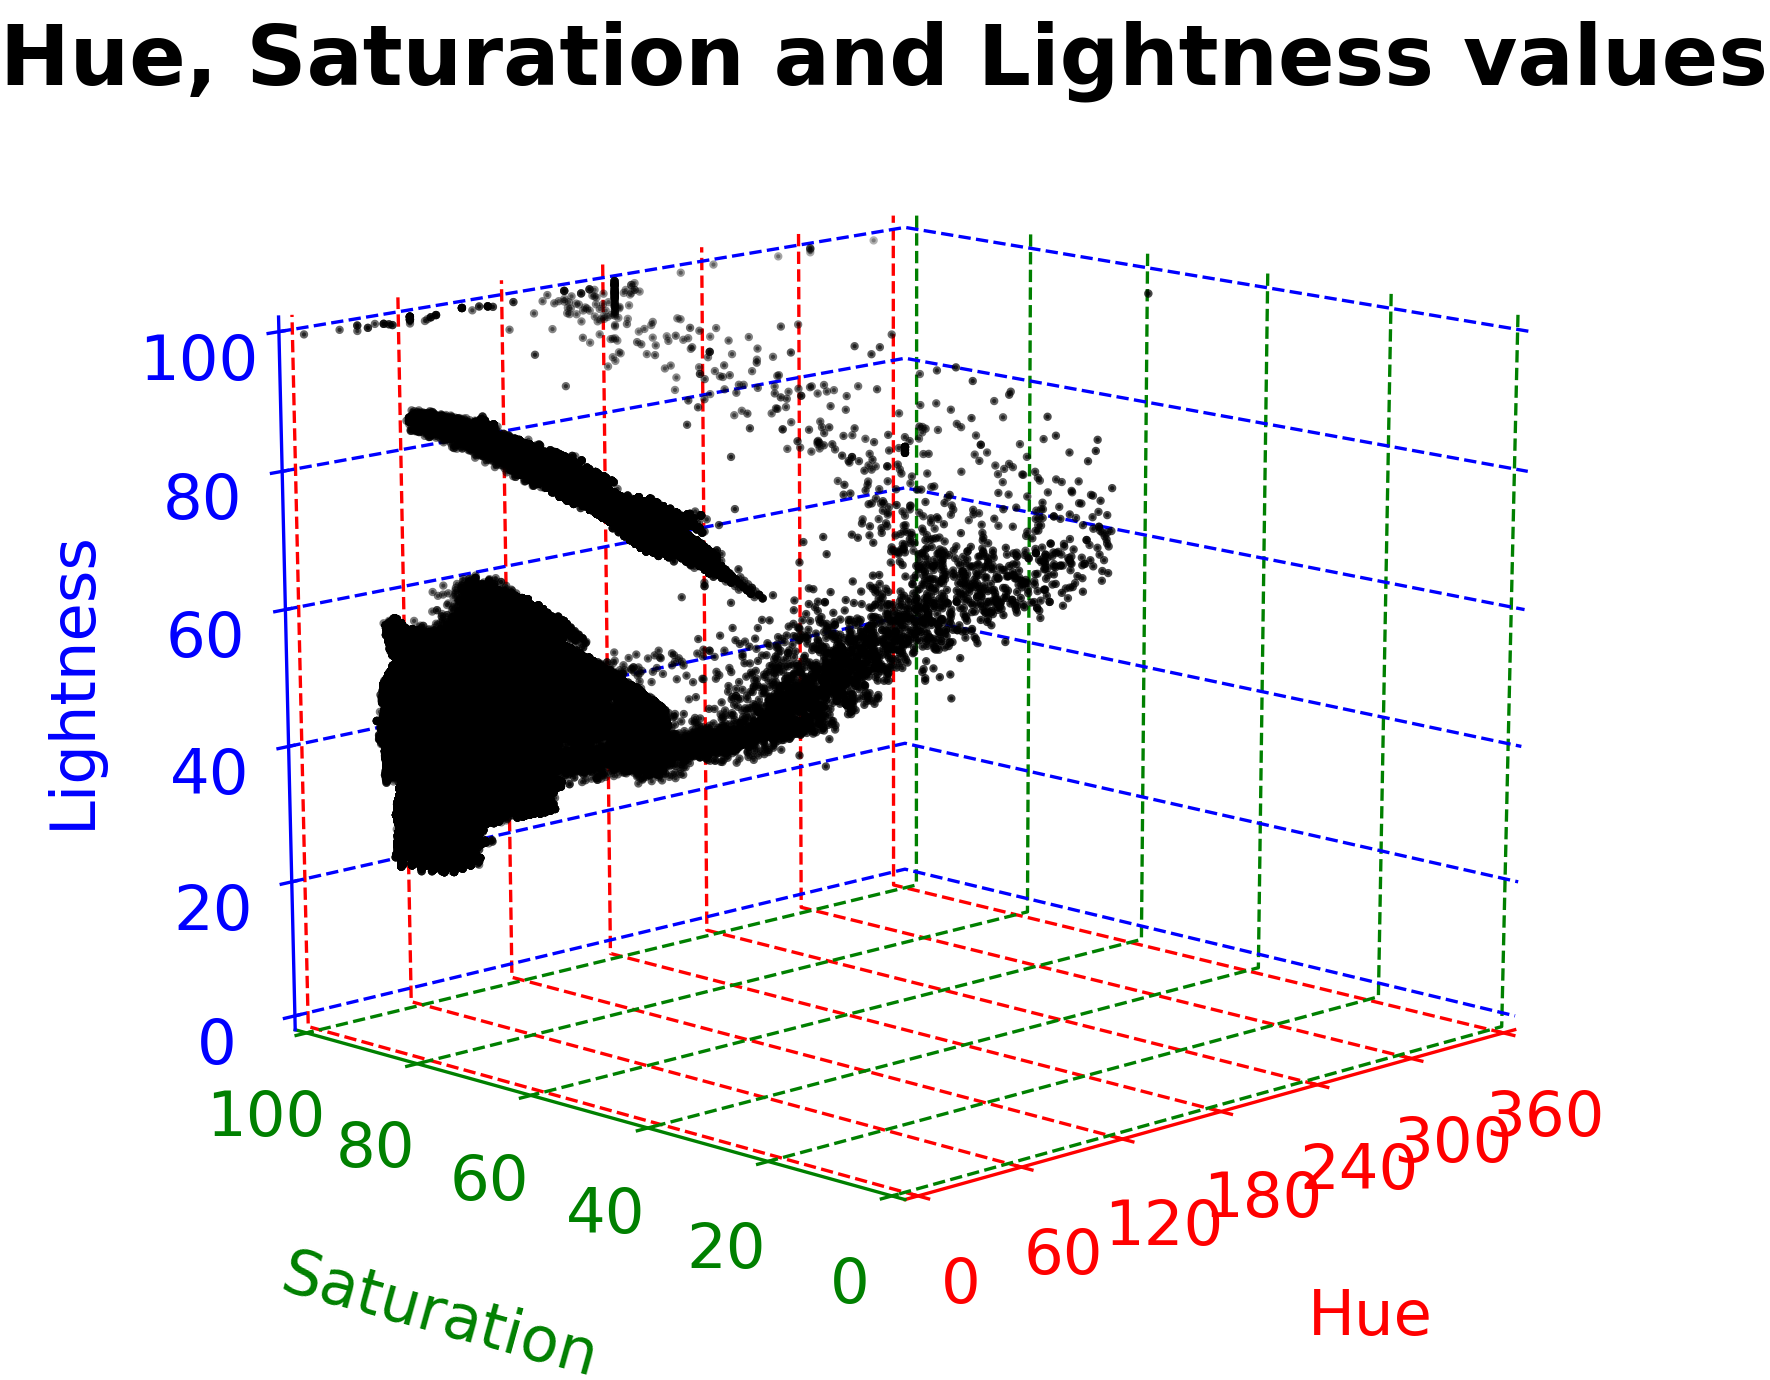
\includegraphics[width=0.9\textwidth]{img/hsl3DYellow.png}
		\captionsetup{width=0.9\textwidth}
		\captionof{figure}{HSL plot voor de kleur geel.}
		\label{hsl3DYellowPlot}
	\end{minipage}
\end{figure}

\vspace{1mm}

\begin{figure}[h!]
	\centering
	\begin{minipage}{0.5\textwidth}
		\centering
		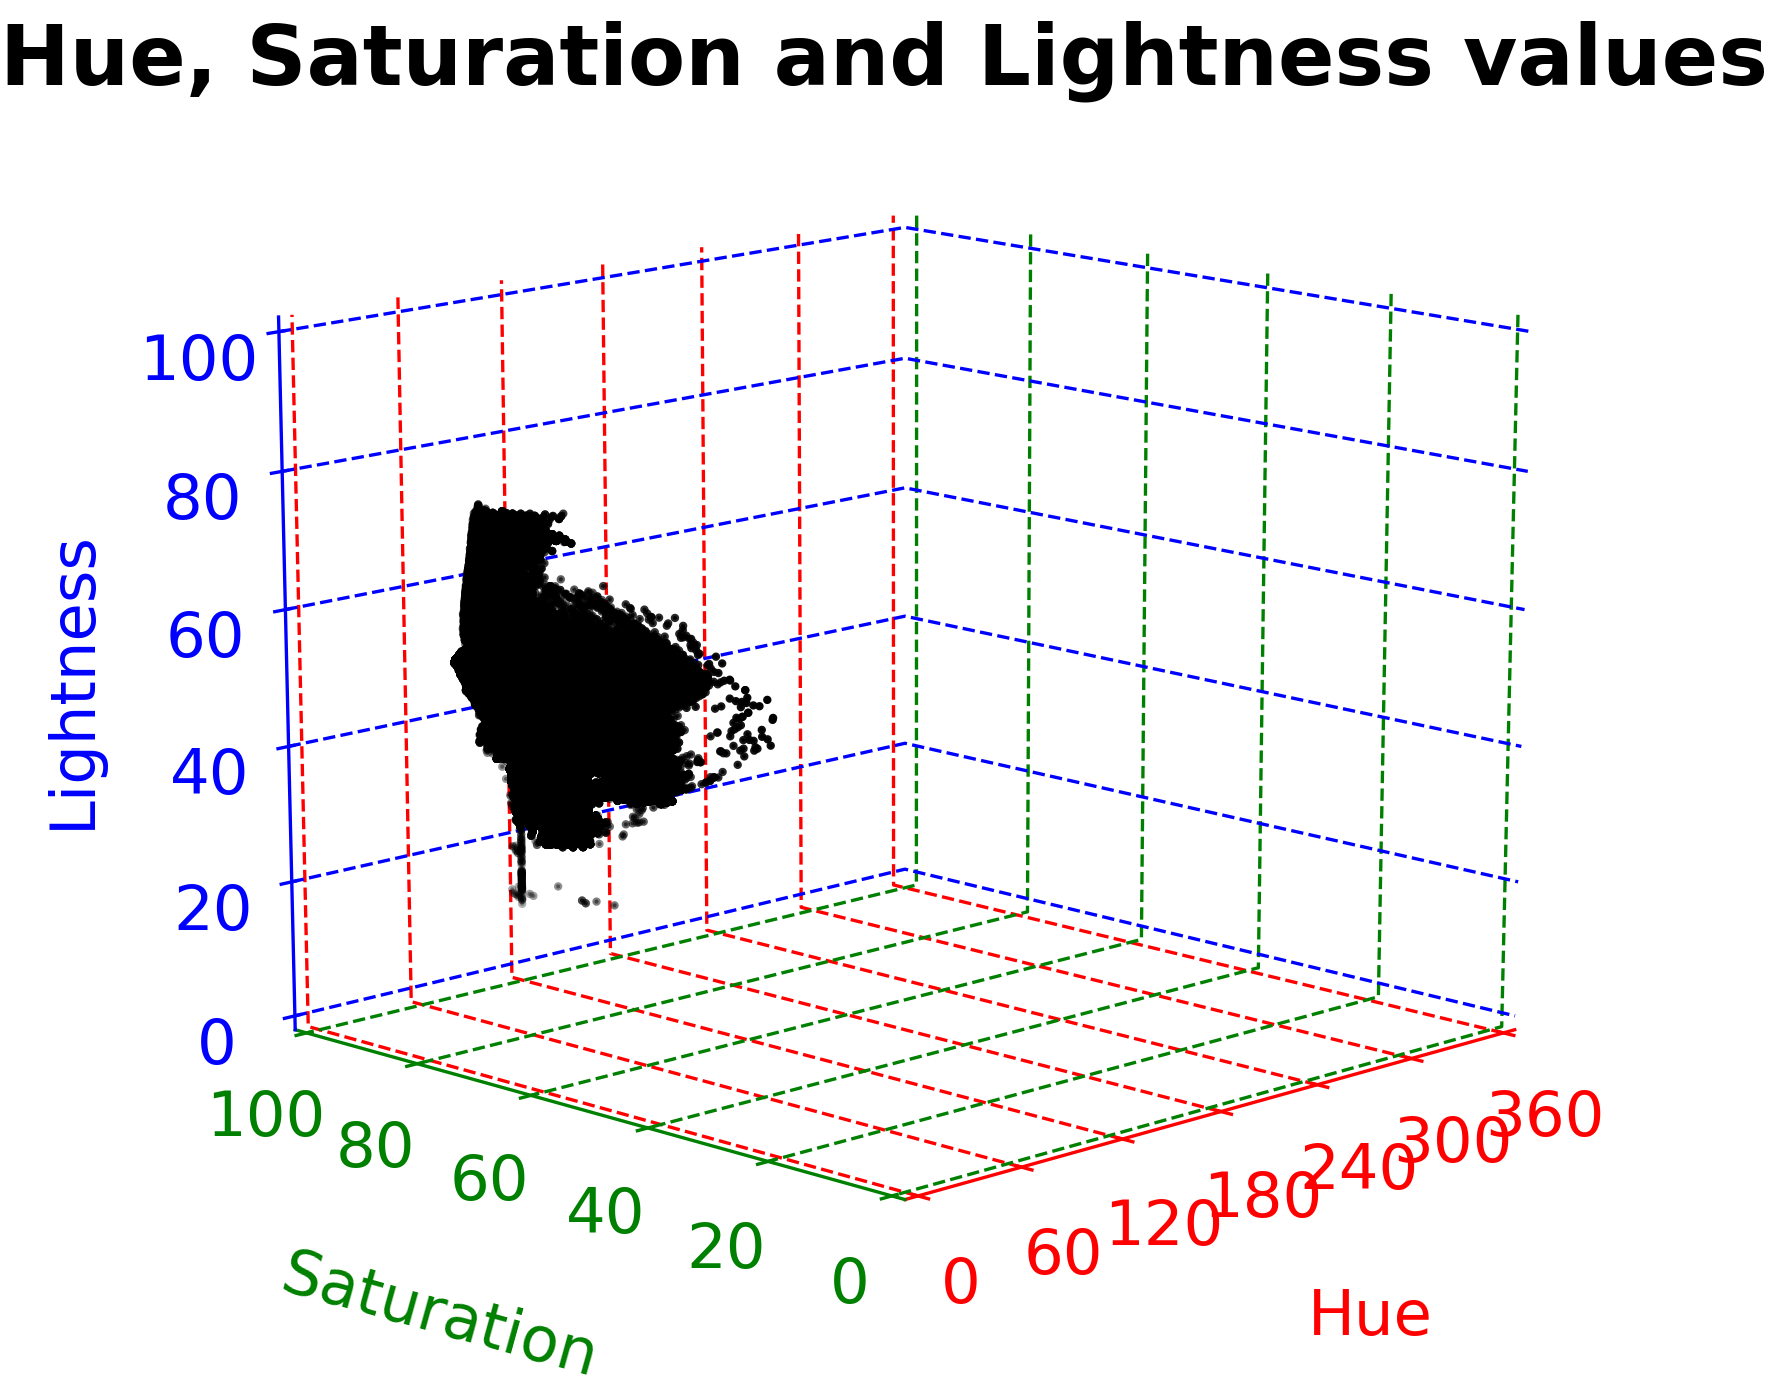
\includegraphics[width=0.9\textwidth]{img/hsl3DGreen.png}
		\captionsetup{width=0.9\textwidth}
		\captionof{figure}{HSL plot voor de kleur groen.}
		\label{hsl3DGreenPlot}
	\end{minipage}%
	\begin{minipage}{0.5\textwidth}
		\centering
		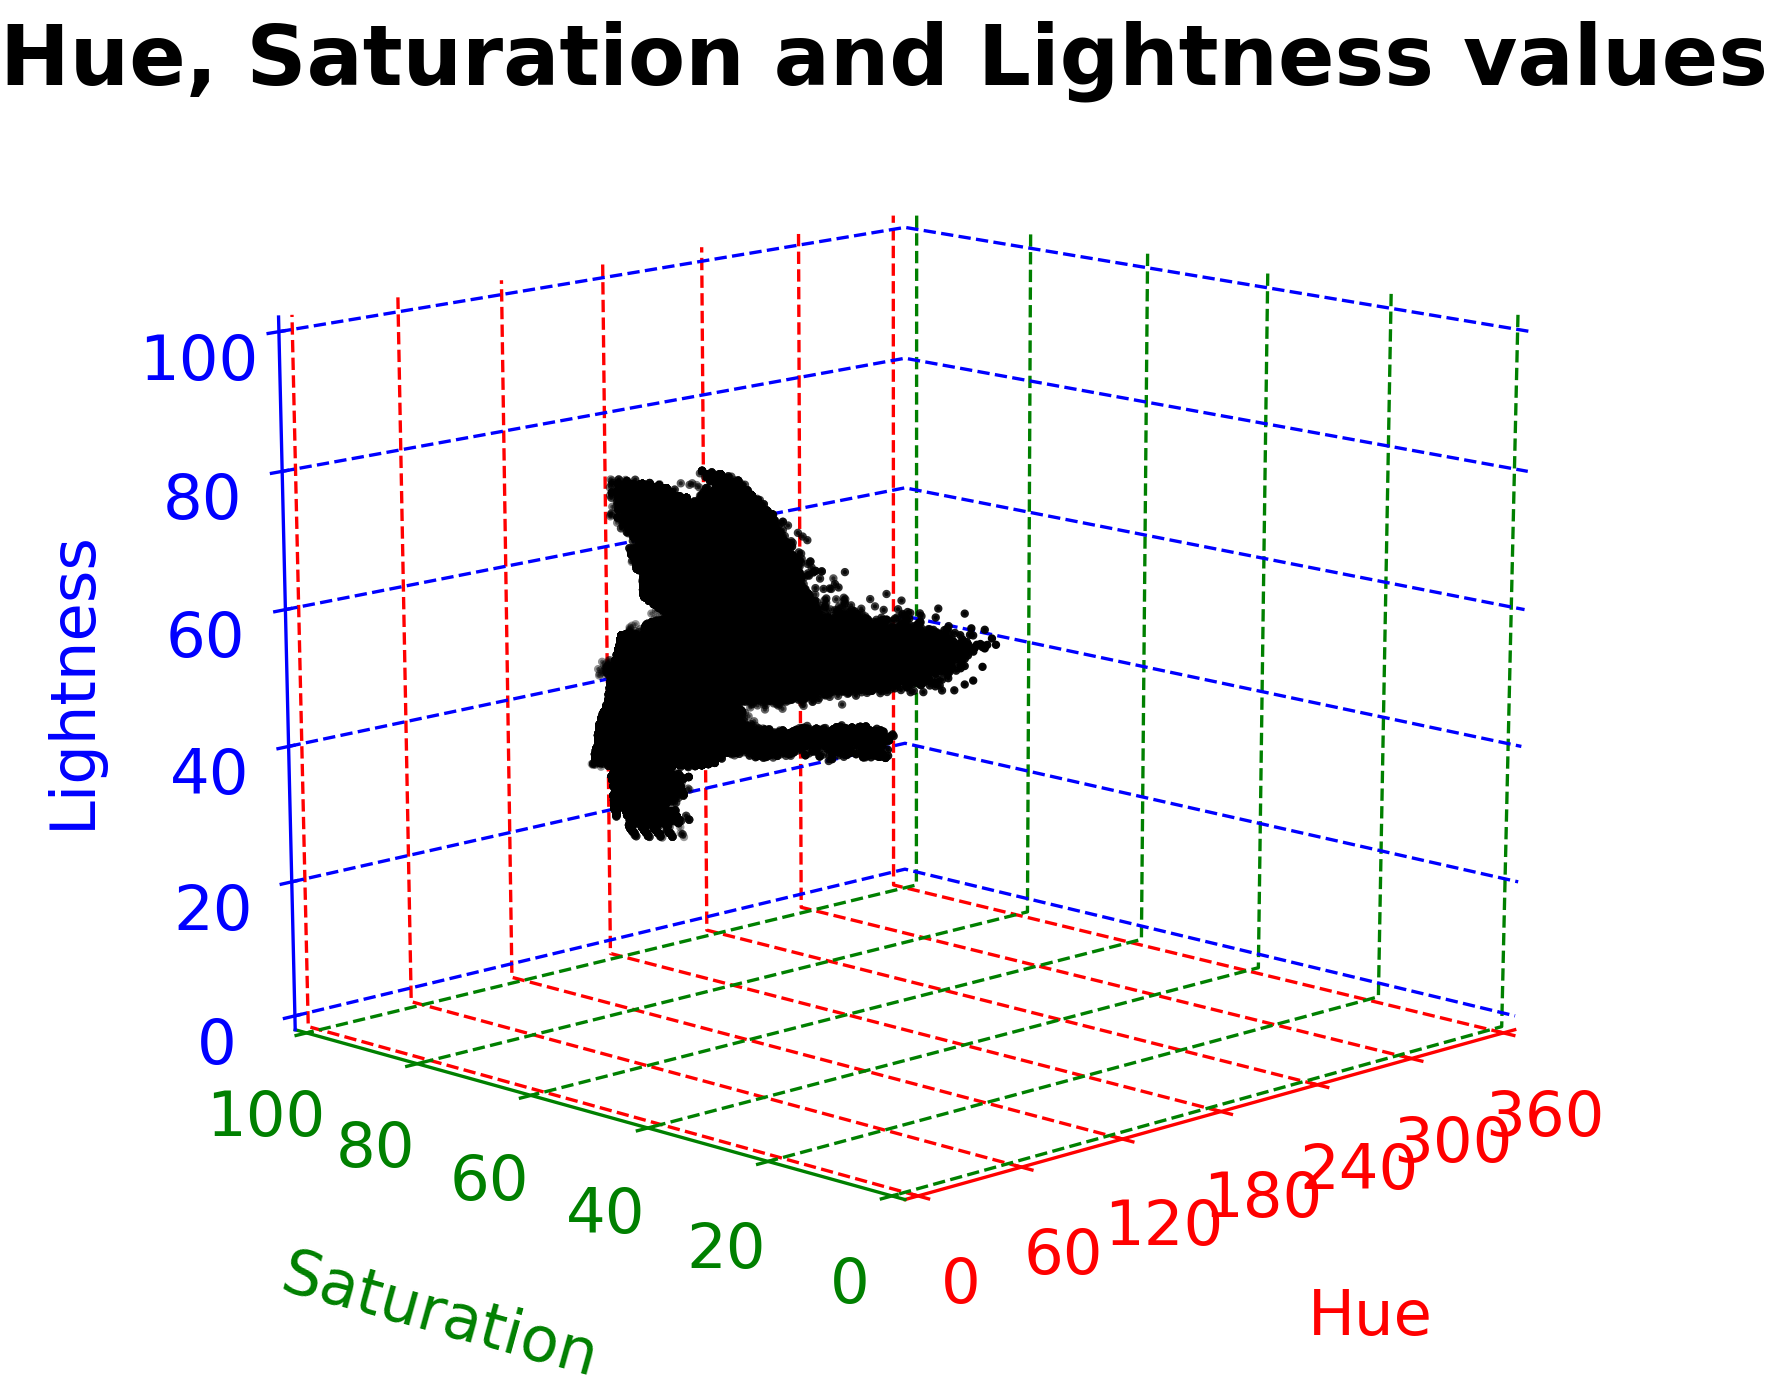
\includegraphics[width=0.9\textwidth]{img/hsl3DBlueGreen.png}
		\captionsetup{width=0.9\textwidth}
		\captionof{figure}{HSL plot voor de kleur cyaan.}
		\label{hsl3DBlueGreenPlot}
	\end{minipage}
\end{figure}

\vspace{1mm}

\begin{figure}[h!]
	\centering
	\begin{minipage}{0.5\textwidth}
		\centering
		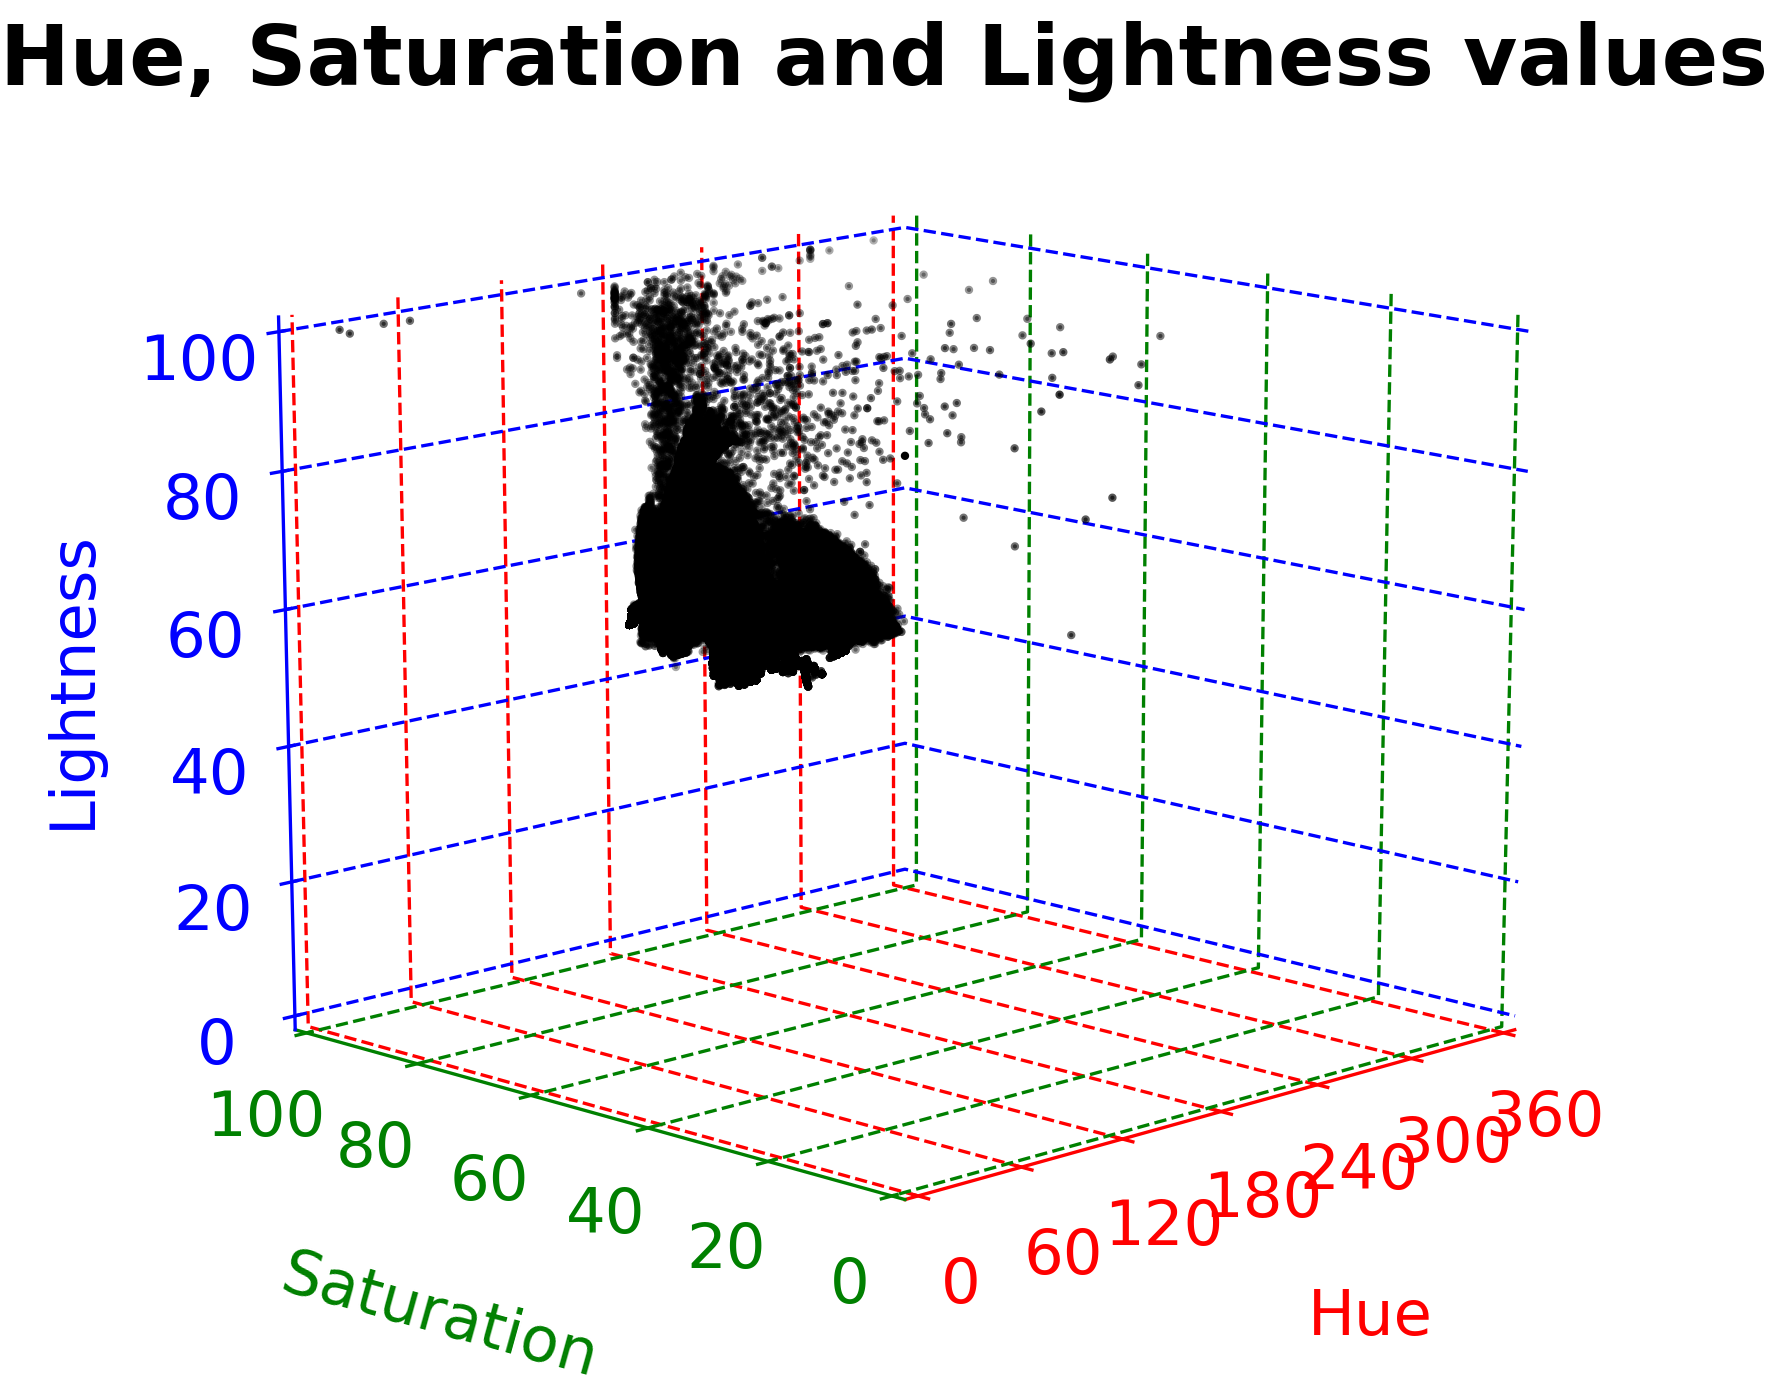
\includegraphics[width=0.9\textwidth]{img/hsl3DBlue.png}
		\captionsetup{width=0.9\textwidth}
		\captionof{figure}{HSL plot voor de kleur blauw.}
		\label{hsl3DBluePlot}
	\end{minipage}%	
	\begin{minipage}{0.5\textwidth}
		\centering
		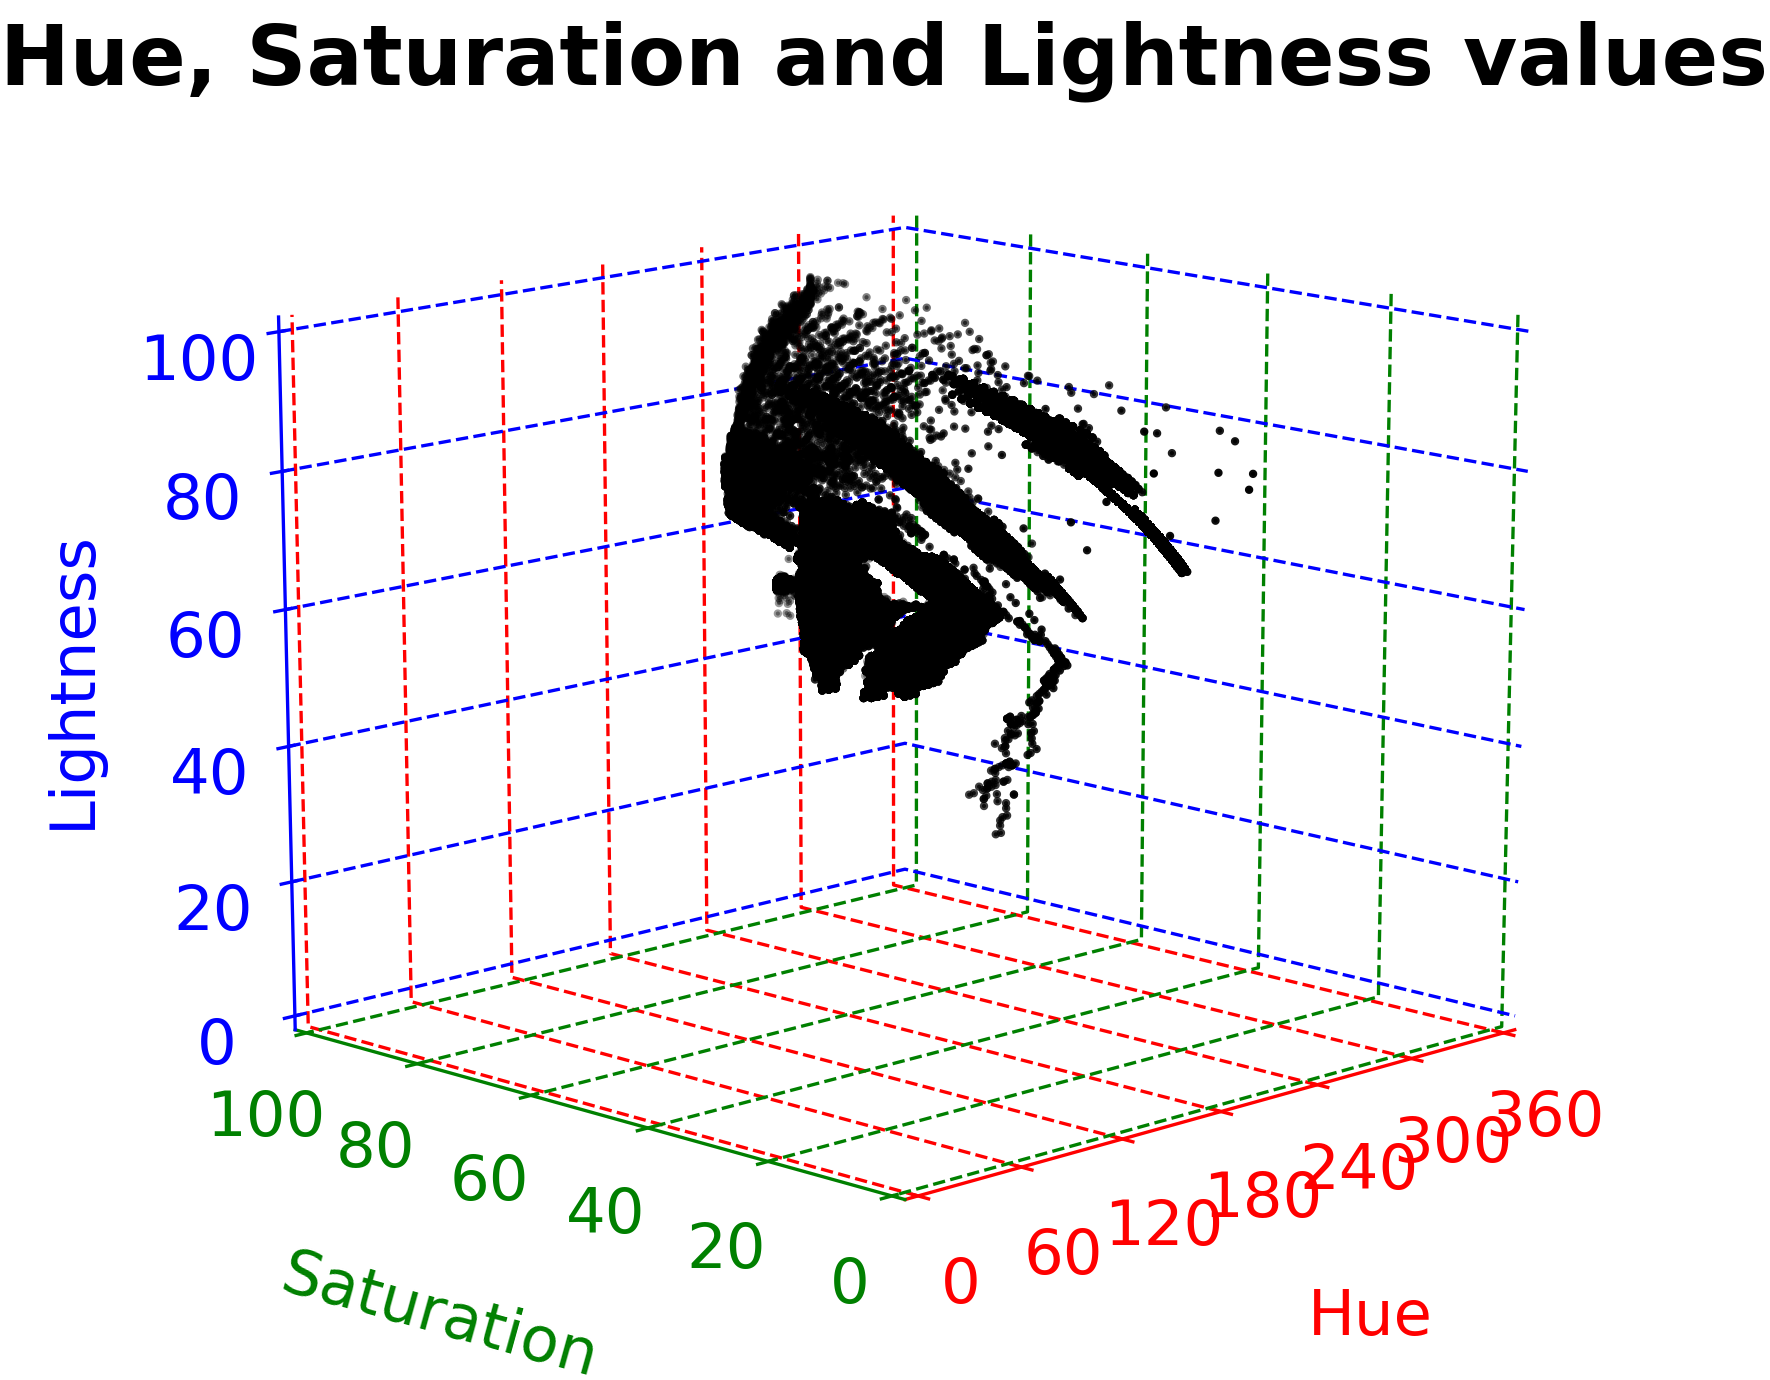
\includegraphics[width=0.9\textwidth]{img/hsl3DPink.png}
		\captionsetup{width=0.9\textwidth}
		\captionof{figure}{HSL plot voor de kleur magenta.}
		\label{hsl3DPinkPlot}
	\end{minipage}
\end{figure}

\subsubsection{2D}

\begin{figure}[h!]
	\center
	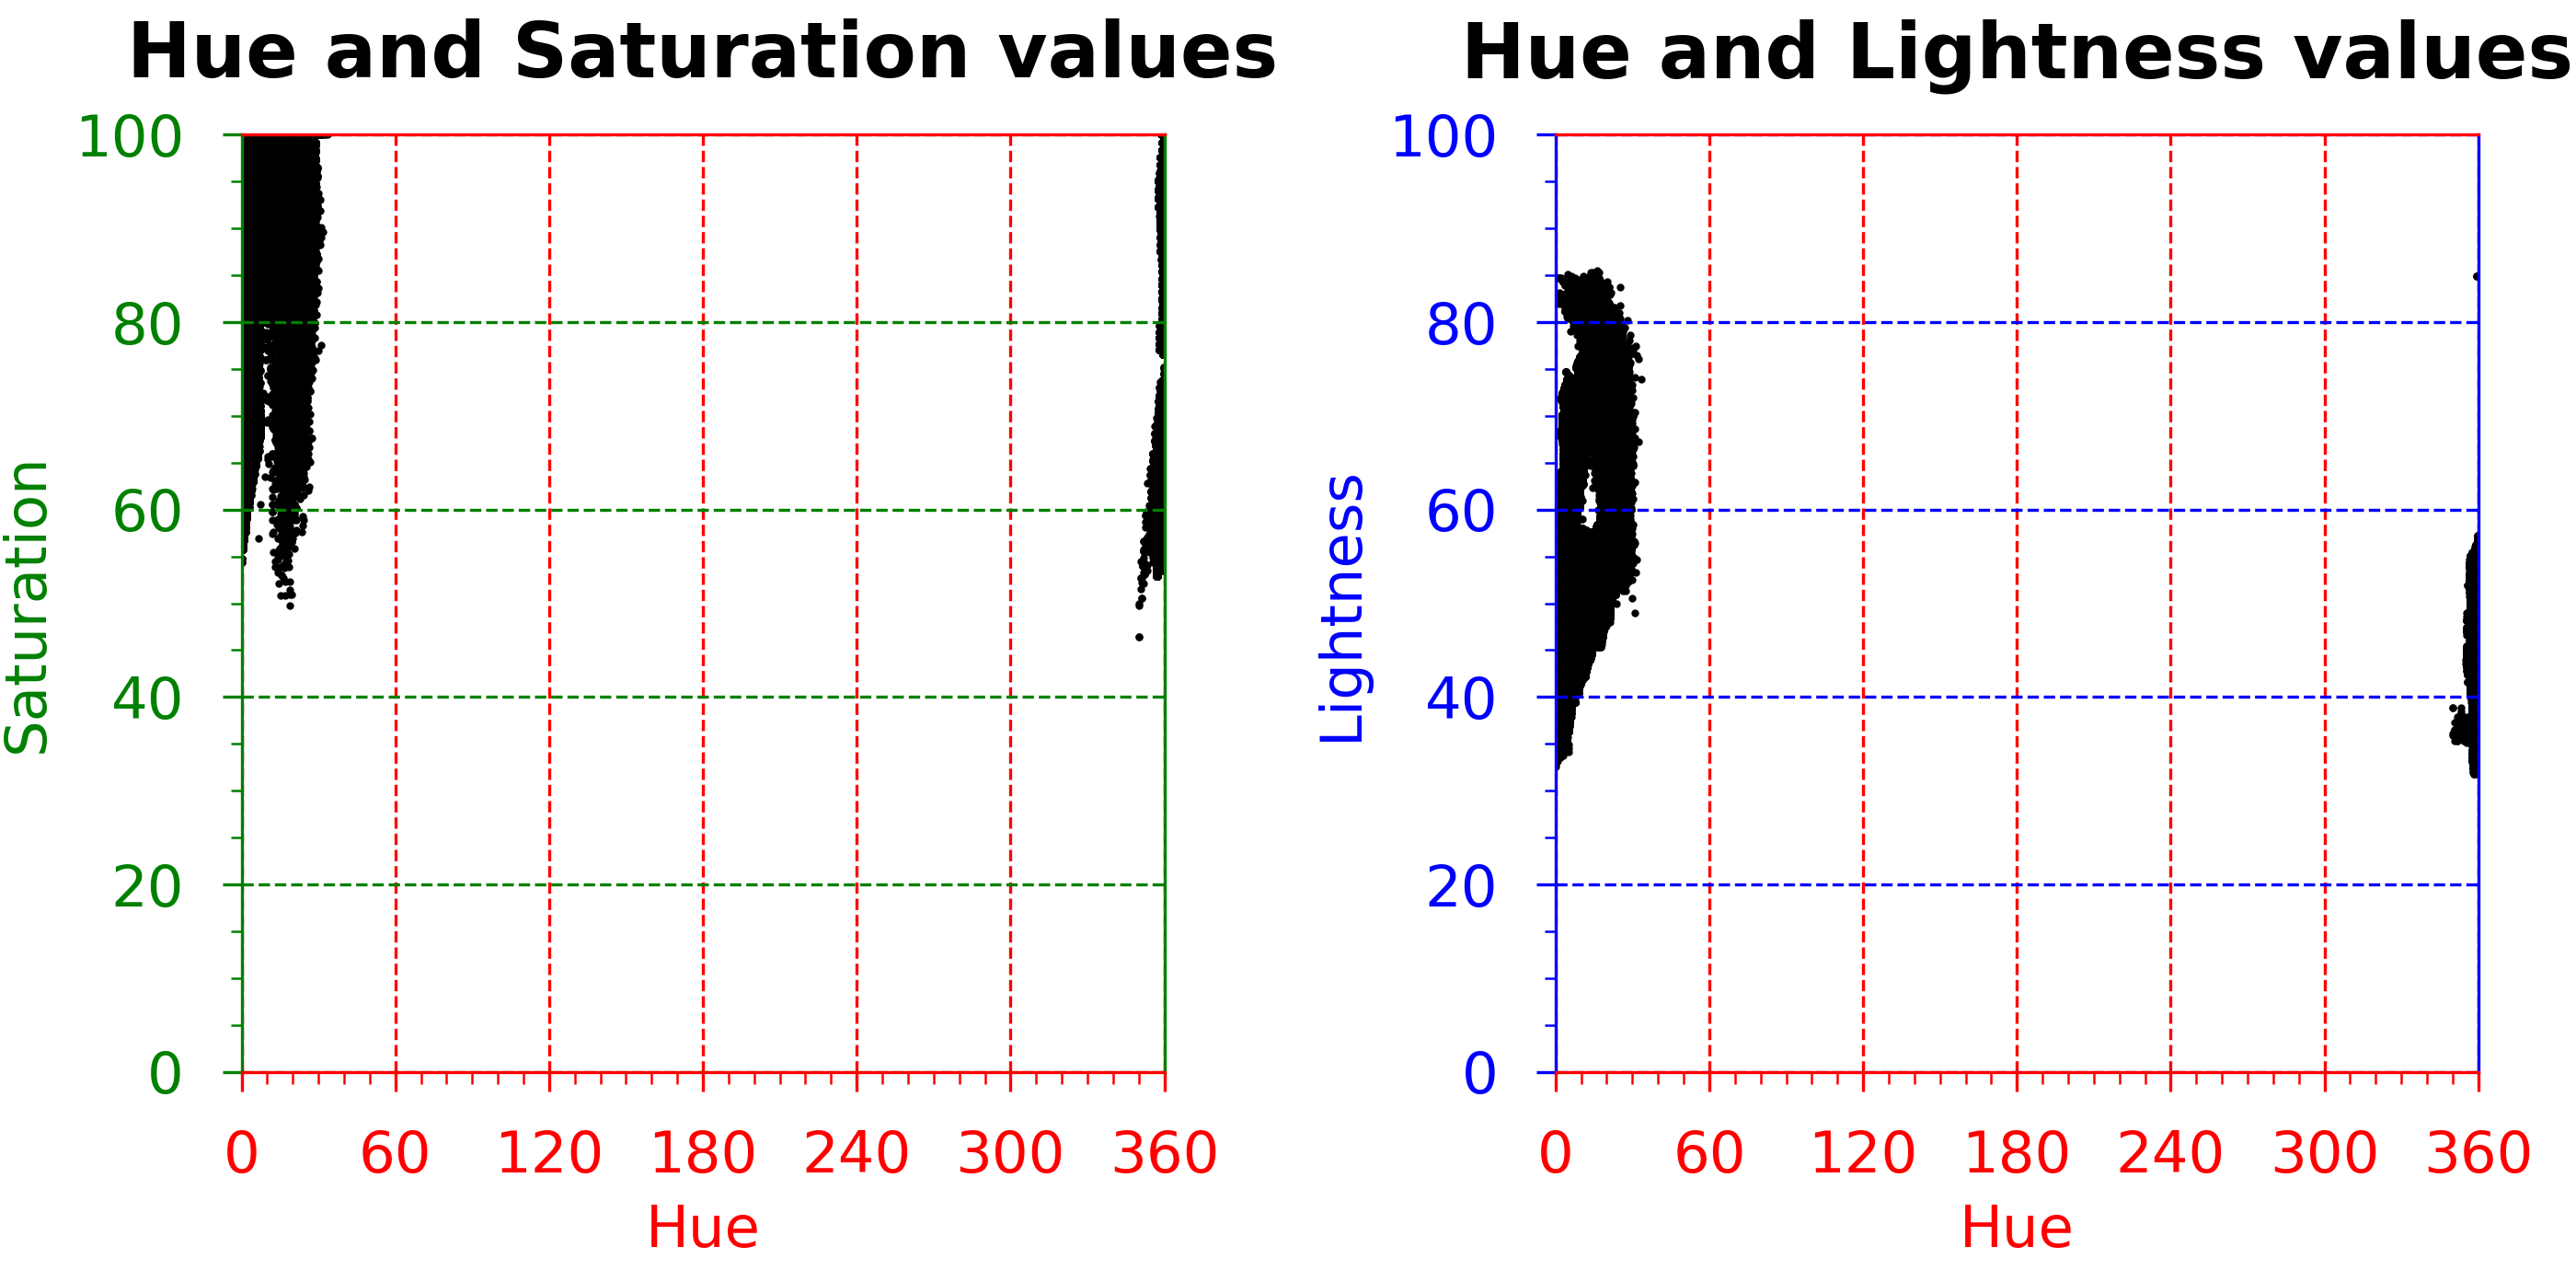
\includegraphics[width=\textwidth]{img/hslRed.png}
	\caption{Scatter plots in functie van tint en saturatie, alsook in functie van tint en lichtheid voor de kleur rood.}
	\label{hslRedPlot}
\end{figure}

\vspace{25mm}

\begin{figure}[h!]
	\center
	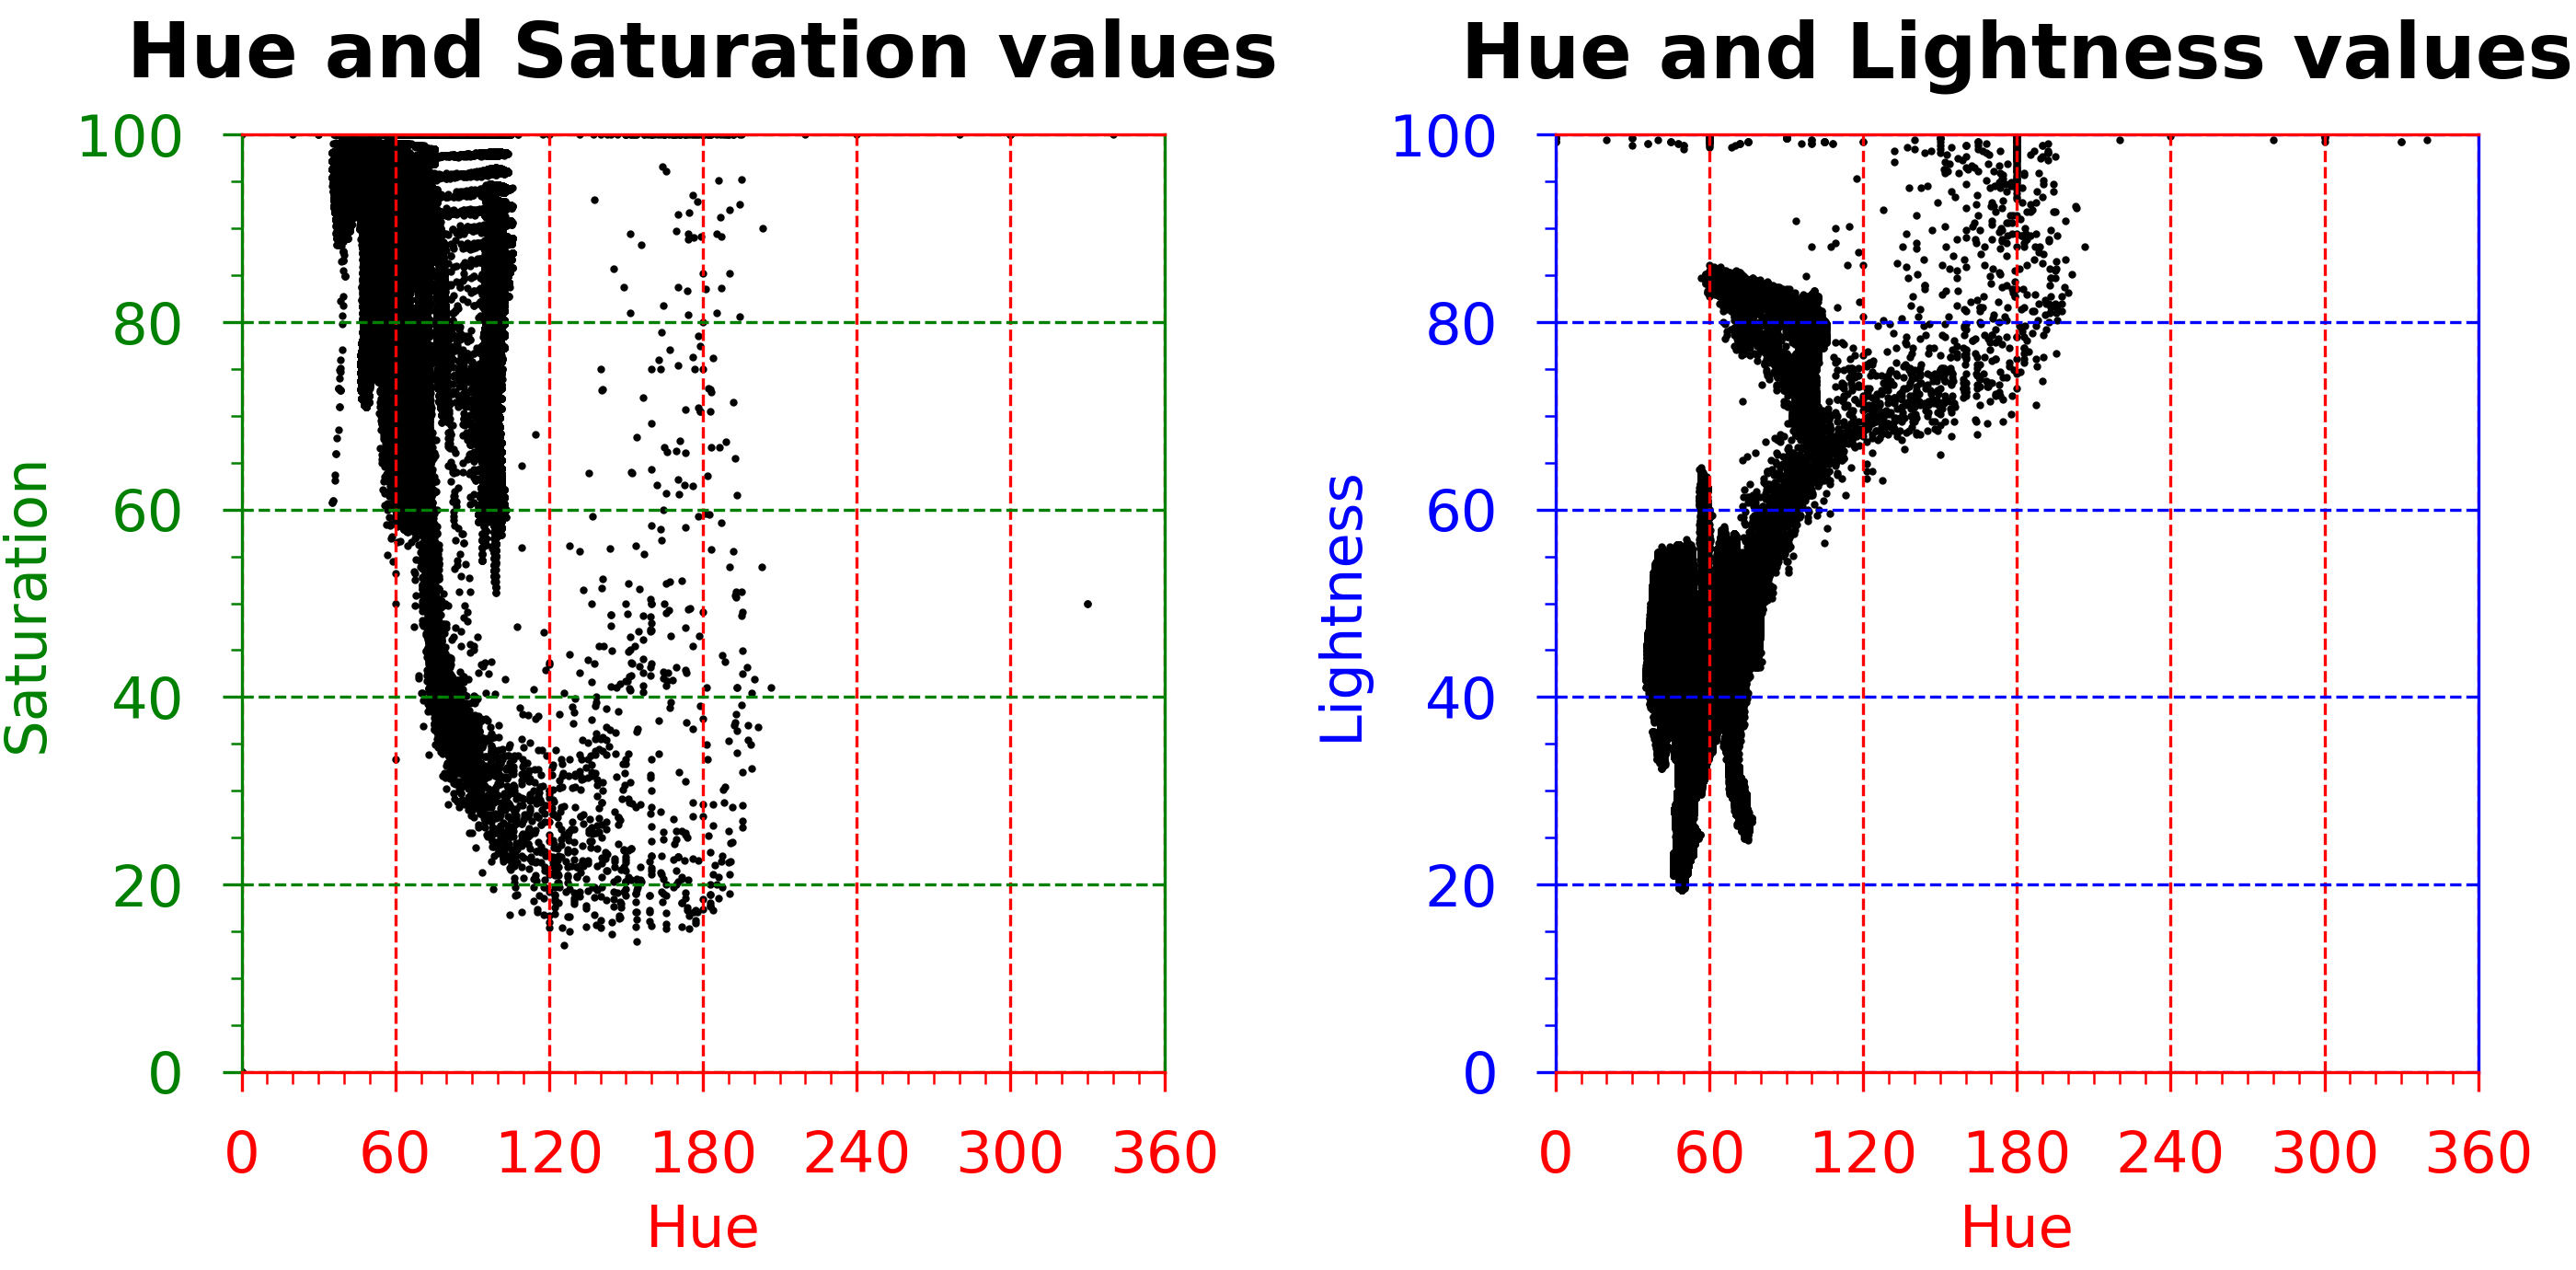
\includegraphics[width=\textwidth]{img/hslYellow.png}
	\caption{Scatter plots in functie van tint en saturatie, alsook in functie van tint en lichtheid voor de kleur geel.}
	\label{hslYellowPlot}
\end{figure}

\begin{figure}[h!]
	\center
	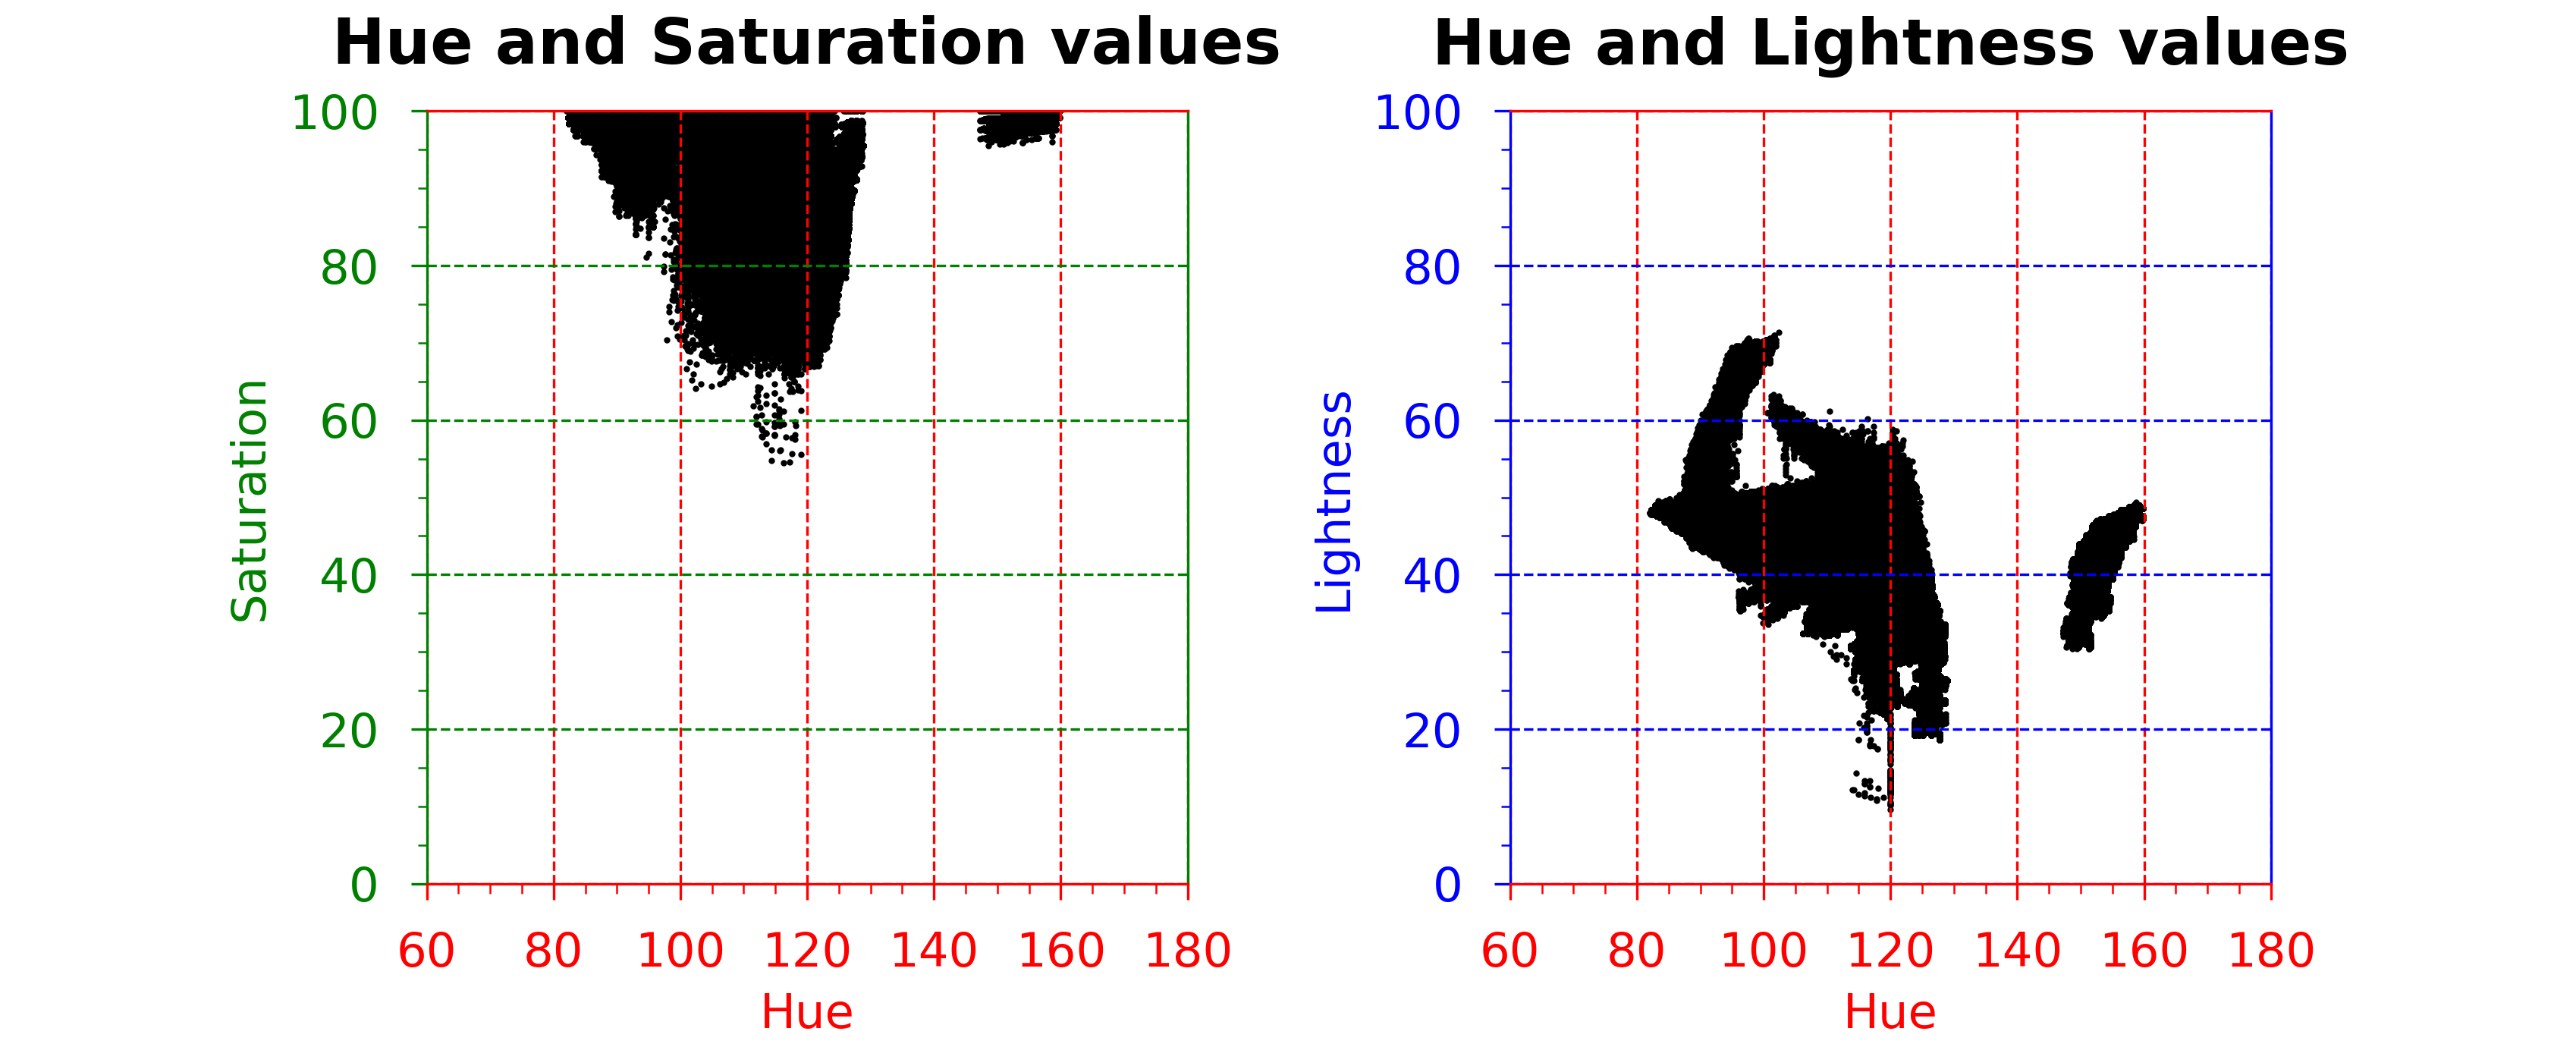
\includegraphics[width=\textwidth]{img/hslGreen.png}
	\caption{Scatter plots in functie van tint en saturatie, alsook in functie van tint en lichtheid voor de kleur groen.}
	\label{hslGreenPlot}
\end{figure}

\begin{figure}[h!]
	\center
	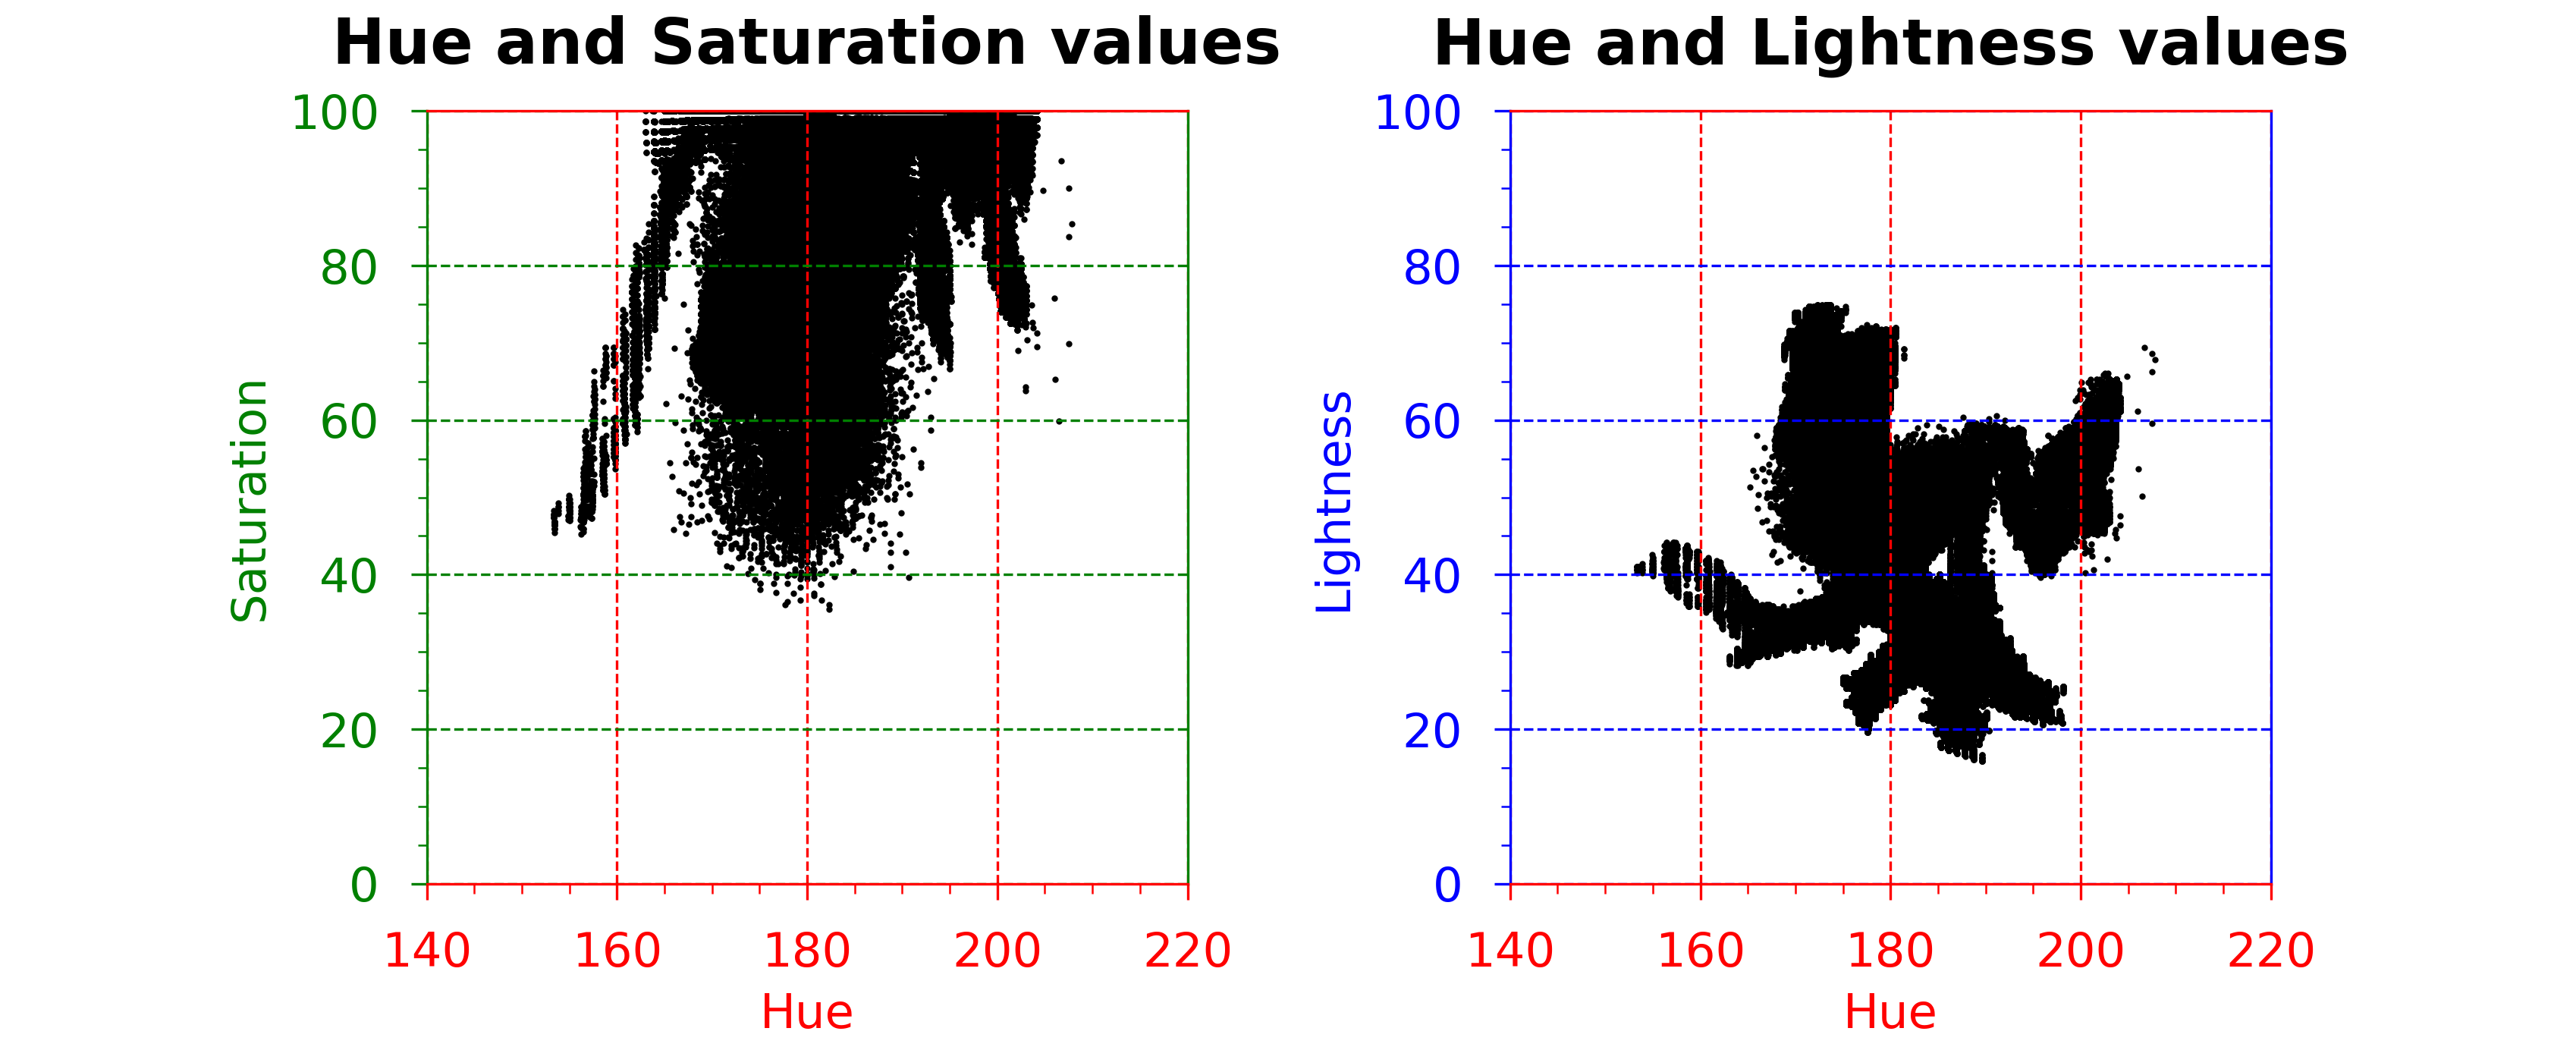
\includegraphics[width=\textwidth]{img/hslBlueGreen.png}
	\caption{Scatter plots in functie van tint en saturatie, alsook in functie van tint en lichtheid voor de kleur cyaan.}
	\label{hslBlueGreenPlot}
\end{figure}

\begin{figure}[h!]
	\center
	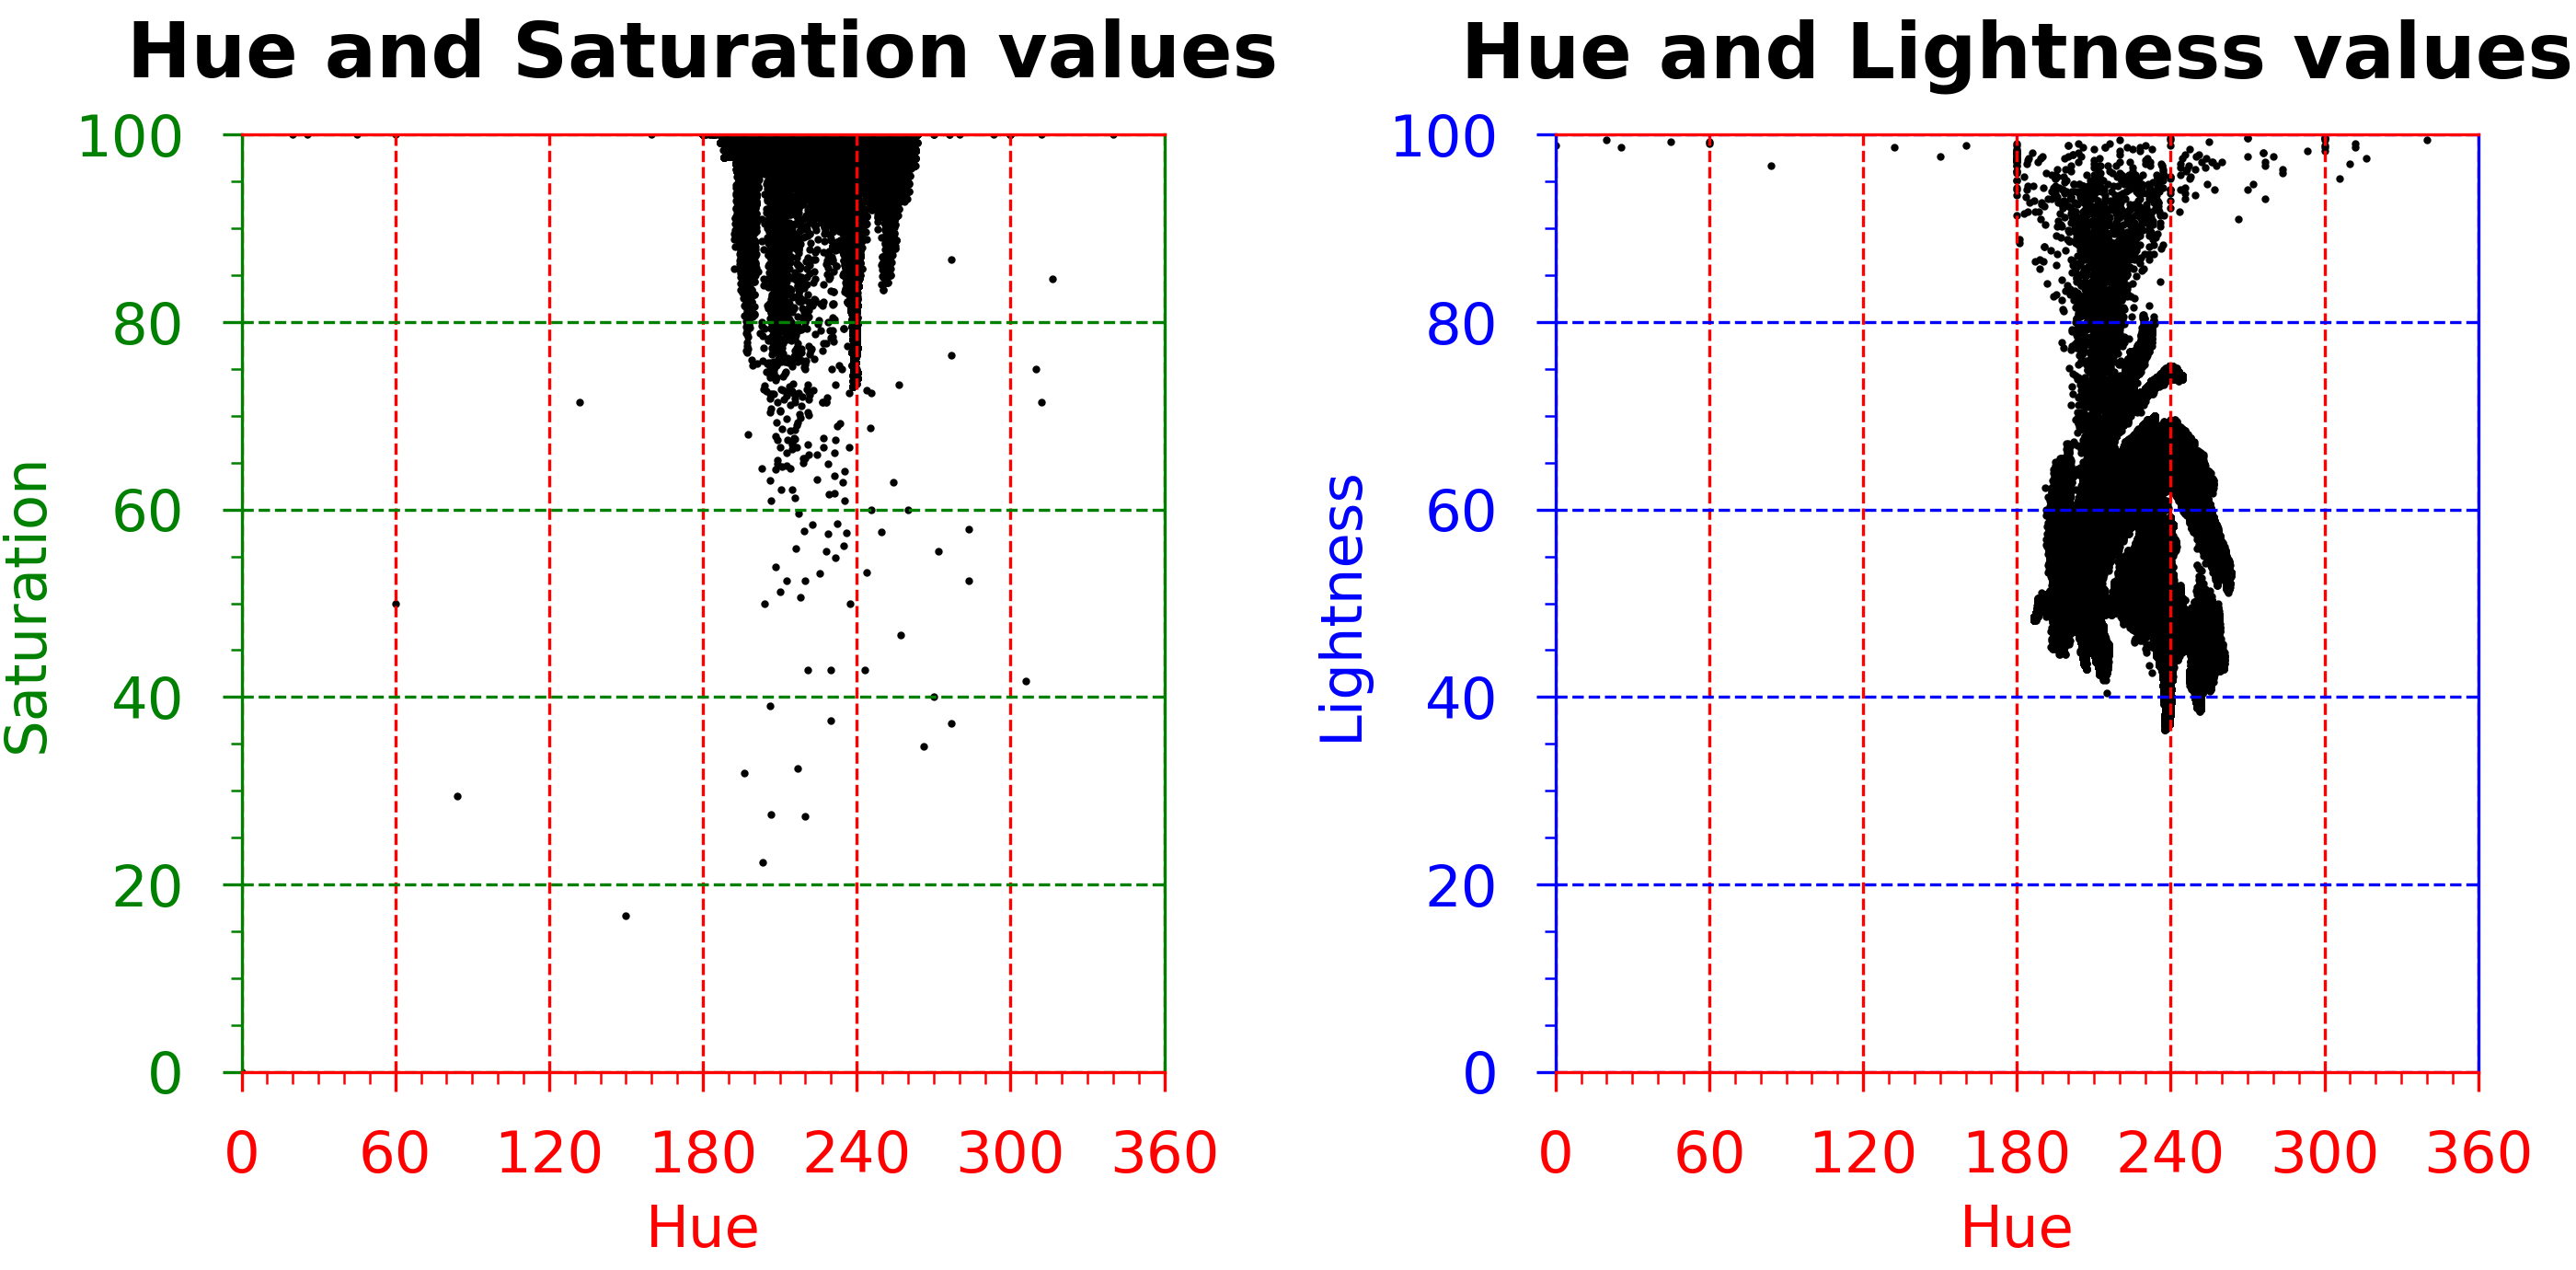
\includegraphics[width=\textwidth]{img/hslBlue.png}
	\caption{Scatter plots in functie van tint en saturatie, alsook in functie van tint en lichtheid voor de kleur blauw.}
	\label{hslBluePlot}
\end{figure}

\begin{figure}[h!]
	\center
	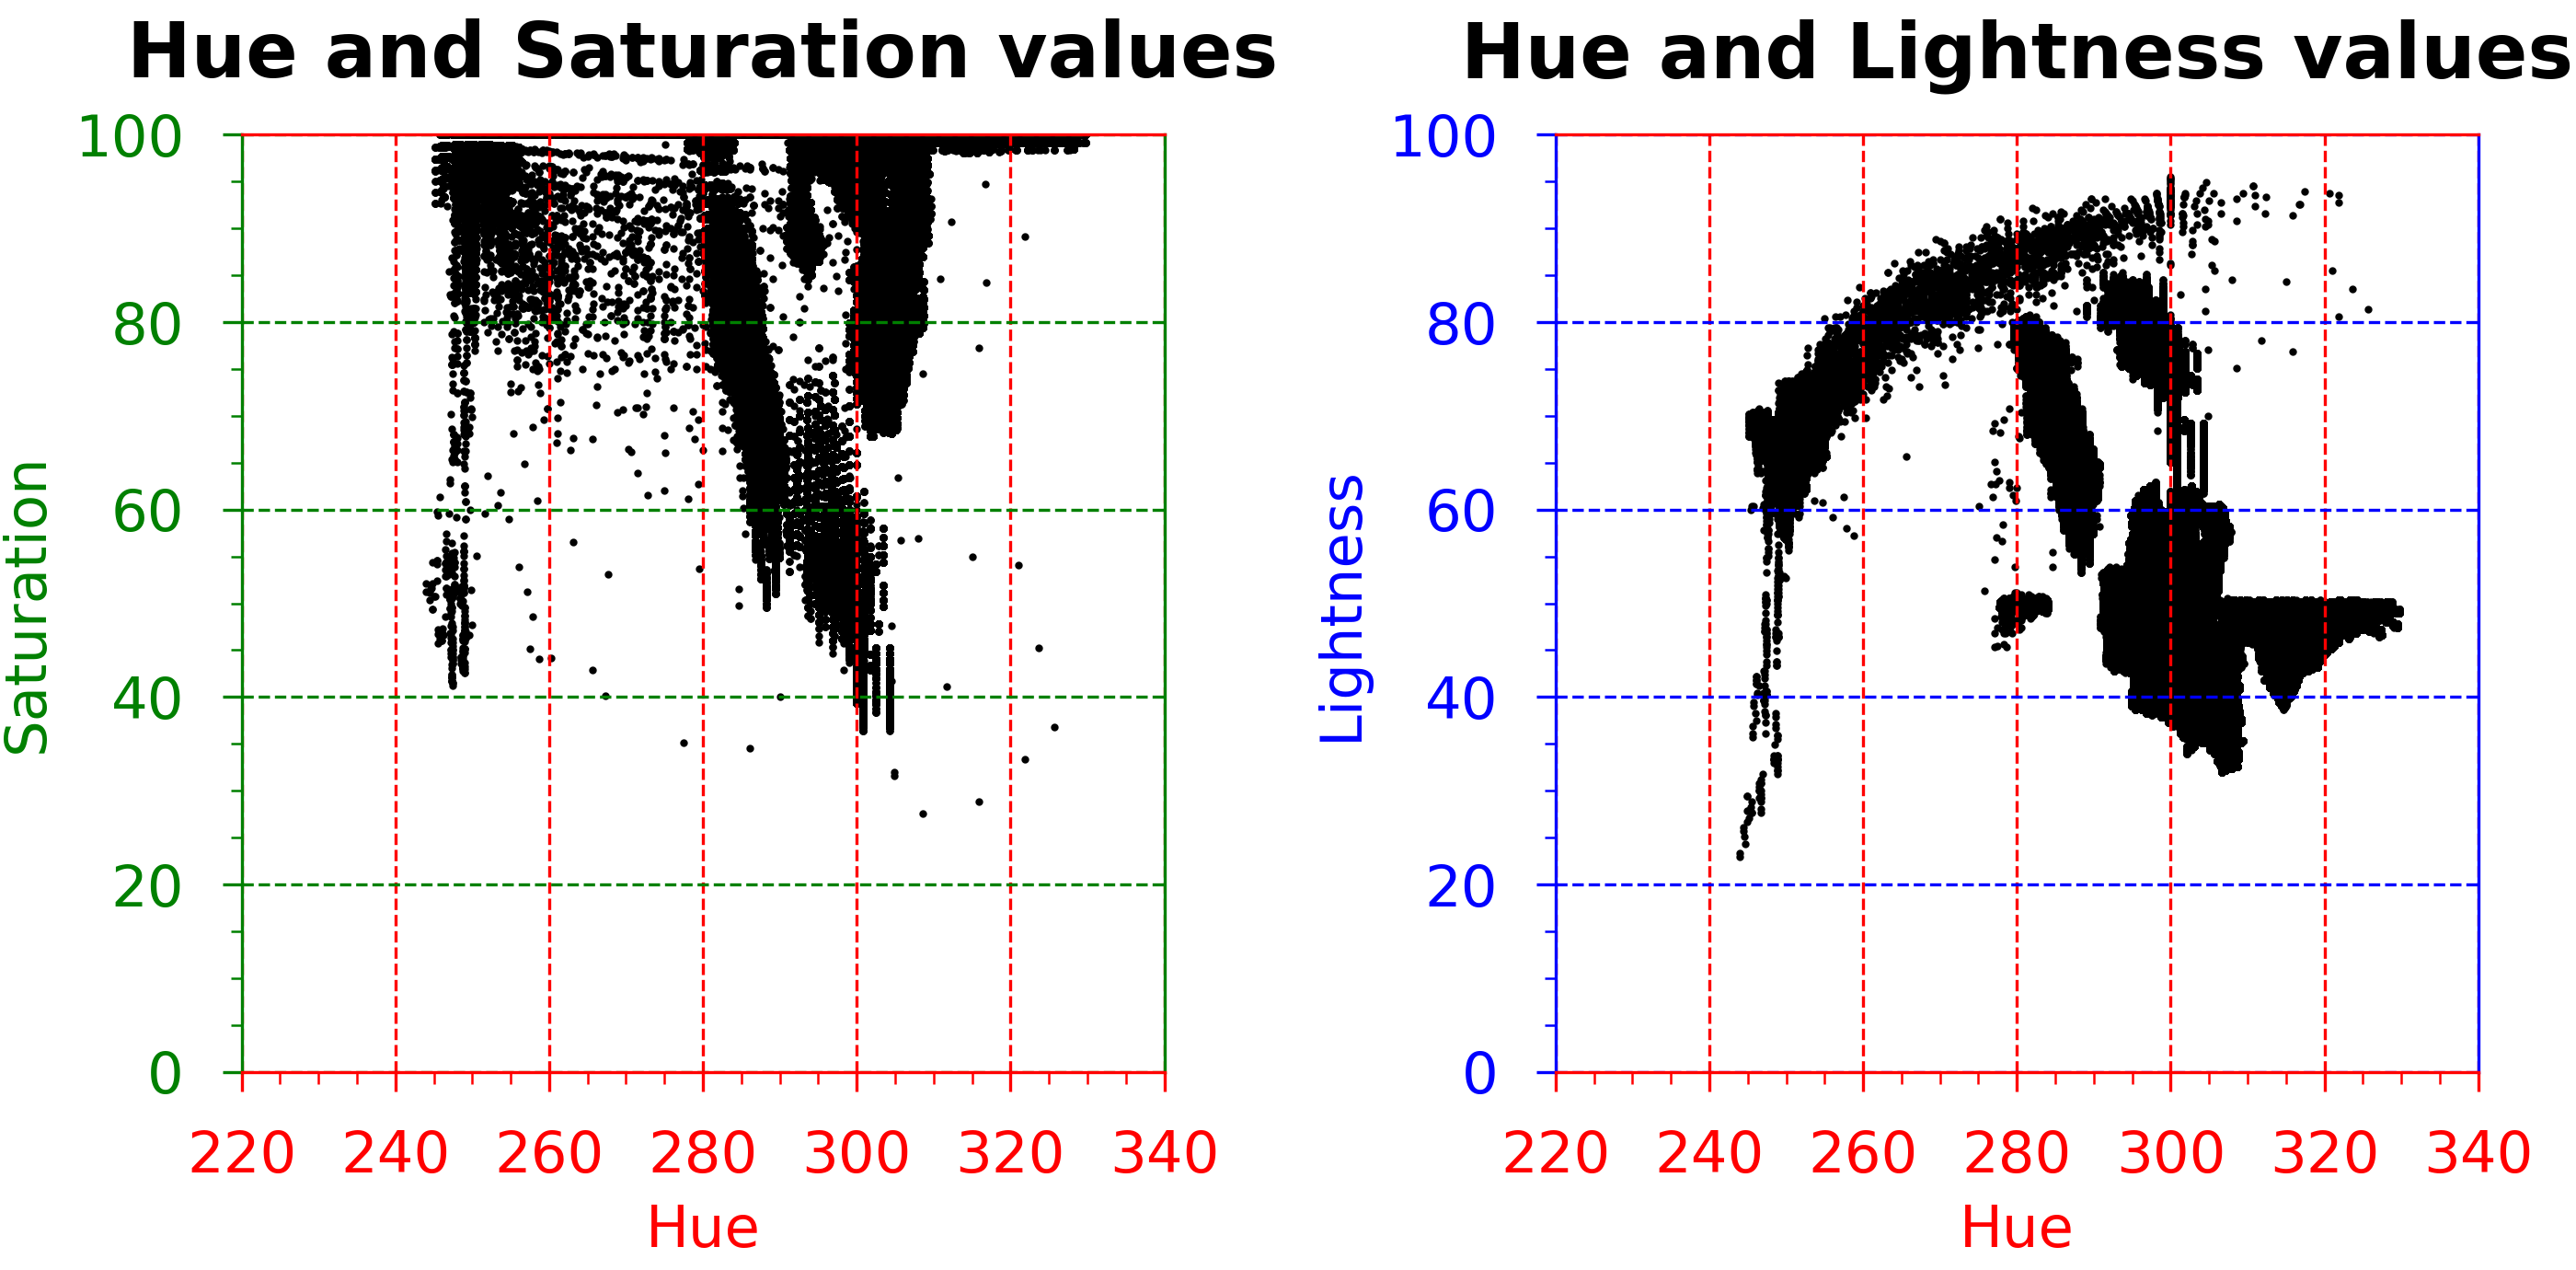
\includegraphics[width=\textwidth]{img/hslPink.png}
	\caption{Scatter plots in functie van tint en saturatie, alsook in functie van tint en lichtheid voor de kleur magenta.}
	\label{hslPinkPlot}
\end{figure}
